% ========================================================================
% CHAPTER 4 — RESULTS (V2 skeleton, Apr 2026)
%
% Purpose of this chapter (UiO Results pattern):
%   Build (what was measured and why), what's new (how this result adds to
%   the state of the art), the result itself (report values, do not
%   interpret).
%
% Content policy:
%   Results describe WHAT. Discussion explains WHY, HOW, and WHAT IT MEANS.
%   Allowed here: metric definitions (by reference to Methods), direction
%   of comparisons, comparison to pre-registered thresholds, outlier
%   flagging, cross-references. Not allowed here: noise models, mechanism
%   hypotheses, literature comparison, synthesis across questions,
%   limitations, clinical implications.
%
% Structural choice: validation-question order under three thematic
%   umbrellas. Umbrella sections (4.1, 4.2, 4.3) give readers the
%   three-thread narrative; Q-numbered subsections preserve the 1:1
%   mapping from Methods Chapter 3 §3.5.
%
% Validation-question renumbering (Apr 2026):
%   new Q1 = EMG front-end characterization (was Q2)
%   new Q2 = EDA front-end characterization (was Q3)
%   new Q3 = Isolation stage characterization (was Q1)
%   Q4 through Q7 unchanged.
%   Methods §3.5 renumber deferred to Phase 5 methods edit pass.
%
% V2 build state (May 2026, post-cascade):
%   25 Main plots saved to Figures/results/.
%   Q7 = 5 plots including per-session signal traces (P5).
%   Pooling convention locked: per-epoch arrays combined across S3-5,
%   reported as pooled mean +/- SD for Q5, Q5b, Q6, Q6b. Q7 reports
%   per-session aggregate then mean +/- SD across n=3 sessions. EDA
%   SNR_circuit and SNR_local follow the Q7 pattern as session-level
%   scalars (no per-epoch arrays).
%   Anchor numbers live in validation_analysis_v2.ipynb stdout. The
%   anchor reference document is Analysis/anchor_reference_v2.md.
% ========================================================================

%\chapter{Results}
\label{ch:results}

This chapter reports the validation measurements obtained from five acquisition sessions following the protocol described in Section~\ref{sec:validation}. Sessions~1 and~2 verified each circuit individually with the other circuit physically disconnected, yielding 120 \gls{emg} contraction epochs from Session~1 and 30 \gls{eda} epochs from Session~2 across the pre- and post-isolation channels. Sessions~3 to~5 acquired \gls{emg} and \gls{eda} simultaneously on the post-isolation channels through three sequential blocks: an EDA-only block, an EMG-only block, and a Combined block. Across all sessions, 360 \gls{emg} contraction epochs and 90 \gls{eda} epochs were acquired. The bystander analyses described in Sections~\ref{sec:results-q5b} and~\ref{sec:results-q6b} use derived epochs from the Sessions~3 to~5 recordings, with epoch counts reported in those sections.

The chapter is organized around the seven validation questions defined in Section~\ref{sec:validation_Q}. Section~\ref{sec:results-frontend} reports the front-end and isolation-stage characterization. Section~\ref{sec:results-crosscontamination} reports the cross-modality contamination assessment. Section~\ref{sec:results-reproducibility} reports the per-session reproducibility analysis. Each subsection corresponds to a Methods question, sharing its Q-number (Section~\ref{sec:validation_Q}).

Metric definitions are given in Sections~\ref{sec:emg_processing} and~\ref{sec:eda_processing}. Per-session and aggregate values are reported as mean $\pm$ sample standard deviation. Interpretation of the results is reported in Chapter~\ref{ch:discussion}.

% -----------------------------------------------------------------------------
% Chapter opening (~half page, before any \section)
% -----------------------------------------------------------------------------
%
% Purpose: orient the reader before the numerical sections start. Answers:
%   - What is being reported and from which recordings?
%   - How do the seven validation questions from Methods §3.5 map to this
%     chapter's three umbrella sections?
%   - What does the reader need to hold in working memory while reading?
%
% Recommended content, three paragraphs:
%
% (1) Scope recap. Five acquisition sessions (Session 1 dedicated to EMG pre+post
%     isolation; Session 2 dedicated EDA pre+post isolation; Sessions 3-5
%     simultaneous EMG+EDA post-isolation with EDA-only, EMG-only, and
%     Combined EMG+EDA blocks). Palm validation site. Total 360 EMG
%     contraction epochs and 90 EDA deep-inhalation epochs across all
%     sessions [VERIFY counts against final V2 cell stdout].
%
% (2) Validation question to section mapping. Section 4.1 covers Q1–Q4
%     (front-end and isolation-stage characterization); section 4.2 covers
%     Q5, Q5b, Q6, Q6b (cross-contamination and coupling); section 4.3
%     covers Q7 (reproducibility). Each Q has its own subsection numbered
%     to match Methods §3.5.
%
% (3) Reporting conventions. Metric definitions are in Methods §3.5.
%     Values here are reported with per-session or aggregate means and
%     sample standard deviations (ddof = 1). Pooling across Sessions 3
%     to 5 combines per-epoch arrays into a single pooled mean +/- SD
%     for Q5, Q5b, Q6, Q6b. Q7 reports per-session aggregate then mean
%     +/- SD across n=3 sessions. EDA SNR_circuit and SNR_local follow
%     the Q7 pattern as session-level scalars. SD bands on multi-epoch
%     overlay plots are a fixed neutral grey (#808080) regardless of
%     condition color. Interpretation of the results appears in
%     Chapter 5.
% -----------------------------------------------------------------------------


% =============================================================================
% 4.1 EMG and EDA Front-End Characterization  (umbrella for Q1-Q4)
% =============================================================================
%
% Umbrella section covering four validation questions on the analog signal
% chain: each front-end's post-isolation characterization (Q1, Q2), the
% isolation stage's cross-modality effect on both signals (Q3), and the
% effect of digital post-filtering on EMG (Q4).
%
% Narrative arc (zoom-in): Q1 characterizes the EMG front-end producing
% contractions visible pre and post isolation → Q2 characterizes the EDA
% front-end producing SCRs visible pre and post isolation → Q3 quantifies
% what the isolation stage adds and preserves across both modalities → Q4
% asks whether digital post-processing can recover EMG signal quality.
% No cross-Q synthesis here — save for Discussion §5.1.
% =============================================================================

\section{Signal Chain Characterization}
\label{sec:results-frontend}

This section reports the characterization of the analog signal chain. The \gls{emg} and \gls{eda} front-ends are characterized post-isolation, the isolation stage is evaluated against pre-isolation data, and digital post-filtering is examined for \gls{emg}. The data are drawn from Sessions~1 and~2, in which each circuit was operated individually.

% Brief "build" paragraph: introduce the signal chain, list which Q covers
% what. One paragraph, ~5 sentences.


% Framing claim (locked): The EMG front-end produces contraction bursts
% visible both pre and post isolation, with quantified post-isolation
% noise floor, contraction RMS, and SNR within the 10-500 Hz design
% bandwidth. Mains harmonic power is reported in §4.1.4 Q4 alongside
% the digital filter response.
% Cross-references:
%   Methods metric definitions: \autoref{sec:methods-q1-emg}
%   Quantitative pre-vs-post comparison: \autoref{sec:results-q3}
%
% Discussion (DO NOT include here):
%   21 µV RMS noise interpretation (Thread Q3.1): §5.1.

\subsection{Q1 - EMG Front-End Characterization}
\label{sec:results-q1}

Figure~\ref{fig:q1-emg-representative} shows a representative single contraction epoch from Session~1, recorded simultaneously on the pre-isolation and post-isolation channels. Contraction bursts during the \SI{1.0}{\second} contraction window are visible on both channels. Section~\ref{sec:results-q3} reports the quantitative comparison of pre- and post-isolation amplitude, frequency content, and waveform morphology.

\begin{figure}[!htbp]
  \centering
  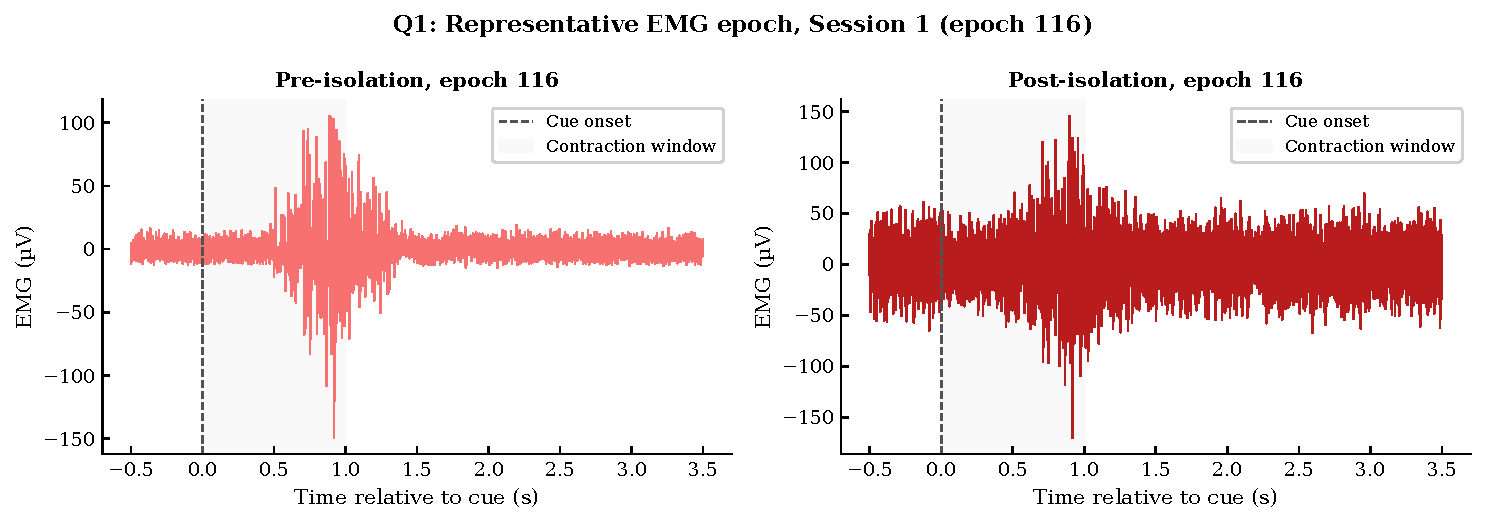
\includegraphics[width=\textwidth]{result_figures/q1_emg_representative_epoch_pre_post.pdf}
  \caption{Representative single contraction epoch from Session~1 (epoch \num{116} of \num{120}), shown on the pre-isolation channel (left) and post-isolation channel (right). Dashed vertical line marks cue onset. Shaded region marks the \SI{1.0}{\second} contraction window.}
  \label{fig:q1-emg-representative}
\end{figure}

The post-isolation noise floor measured across the pre-cue window of the \num{119} contamination-filtered epochs from Session~1 was $\num{21.70} \pm \num{0.99}$\,\si{\micro\volt} \gls{rms}. Contraction-window \gls{rms} was $\num{32.17} \pm \num{4.98}$\,\si{\micro\volt}, and the per-epoch \gls{snr} was $\num{3.32} \pm \num{1.34}$\,\si{\decibel}. Figure~\ref{fig:q1-emg-overlay} shows the envelope across these epochs.

\begin{figure}[!htbp]
  \centering
  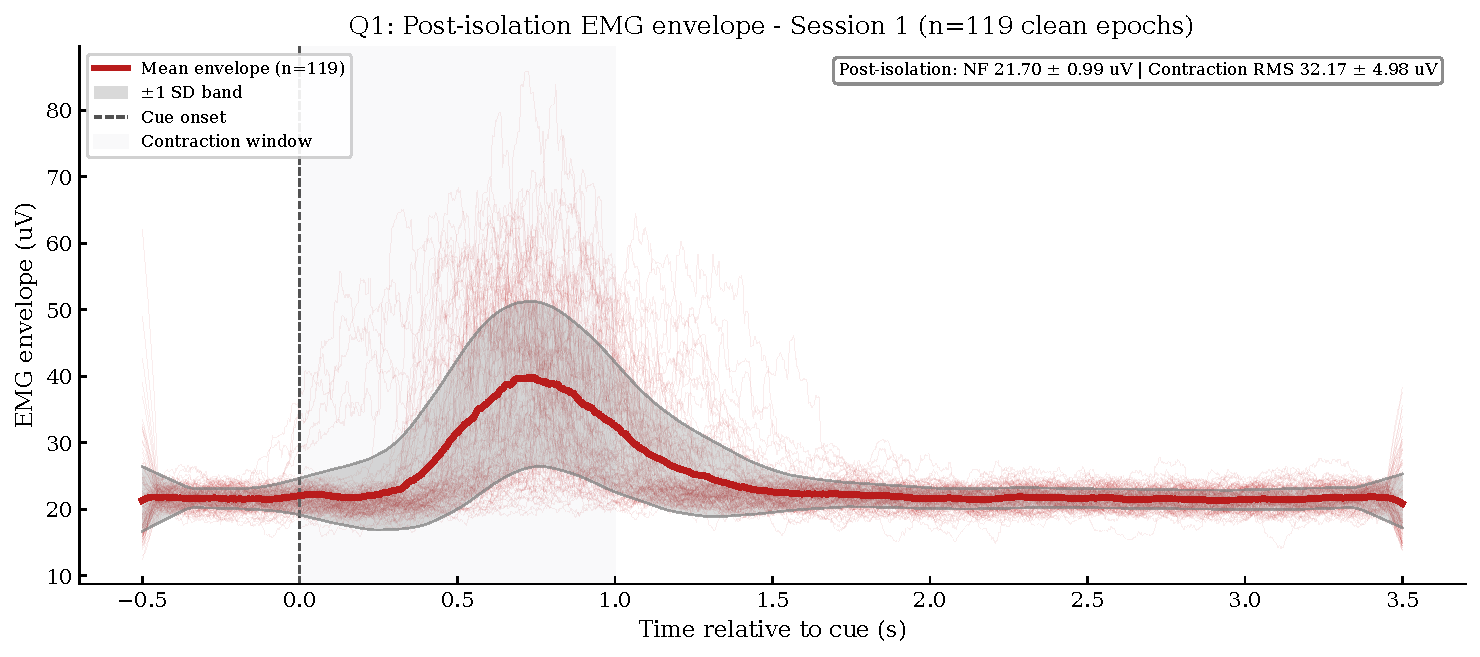
\includegraphics[width=\textwidth]{result_figures/q1_emg_overlay_post.pdf}
  \caption{Post-isolation \gls{emg} envelope across the \num{119} contamination-filtered epochs of Session~1. The solid line shows the across-epoch mean, and the grey band shows $\pm 1$ SD across epochs. Noise floor and contraction-window \gls{rms} are annotated. Light red traces show individual epochs.}
  \label{fig:q1-emg-overlay}
\end{figure}

Figure~\ref{fig:q1-emg-psd} shows the post-isolation \gls{psd}. Table~\ref{tab:q1-emg-metrics} summarizes the per-epoch metrics.

\begin{figure}[!htbp]
  \centering
  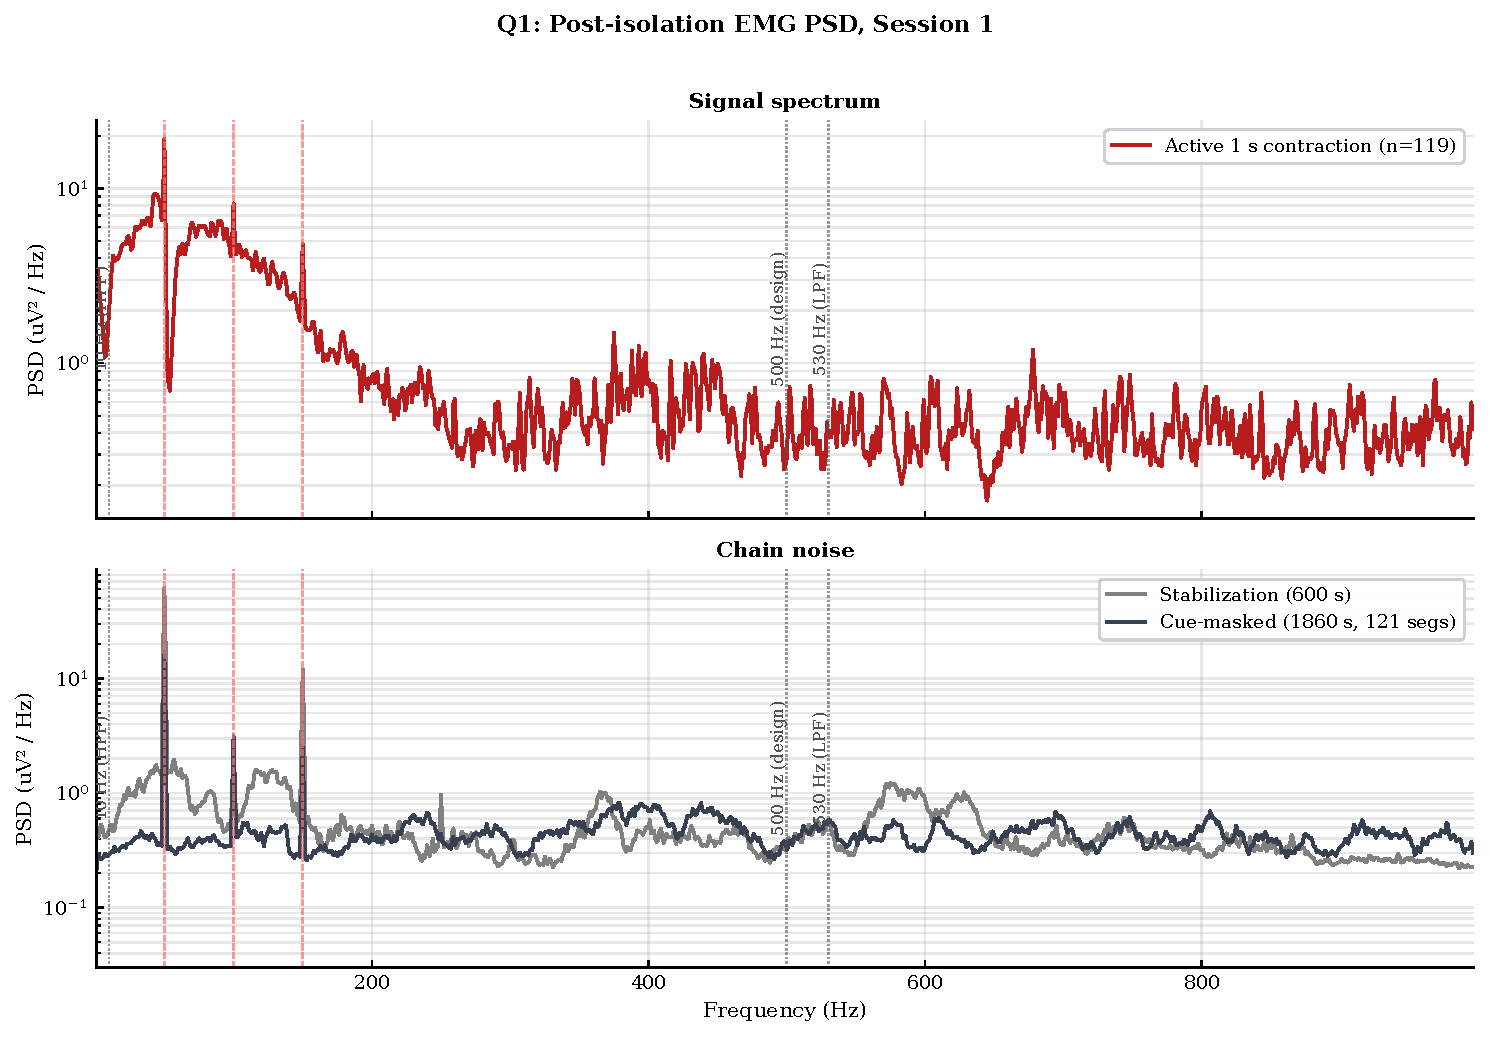
\includegraphics[width=\textwidth]{result_figures/q1_emg_psd.pdf}
  %\caption{Post-isolation \gls{emg} \gls{psd}, Session~1 ($n = \num{119}$ contamination-filtered epochs). Top panel shows the signal spectrum from the active \SI{1.0}{\second} contraction window. The analog \gls{lpf} cutoff at \SI{530}{\hertz} is marked. Integrated band powers at the \SI{50}{\hertz}, \SI{100}{\hertz}, and \SI{150}{\hertz} mains harmonics are annotated. Bottom panel shows the chain-noise spectrum from the cue-masked stabilization windows.}
  \caption{Post-isolation \gls{emg} \gls{psd}, Session~1. Top panel: signal spectrum from the active \SI{1}{\second} contraction window. Bottom panel: chain-noise spectrum from the stabilization and cue-masked windows. Vertical lines mark the analog \gls{hpf} cutoff at \SI{10}{\hertz}, the design bandwidth at \SI{500}{\hertz}, and the analog \gls{lpf} cutoff at \SI{530}{\hertz}.}
  \label{fig:q1-emg-psd}
\end{figure}

\begin{table}[!htbp]
  \centering
  \caption{Post-isolation \gls{emg} metrics, Session~1 ($n = \num{119}$ contamination-filtered epochs).}
  \label{tab:q1-emg-metrics}
  \begin{tabular}{l c l}
    \toprule
    \textbf{Metric} & \textbf{Value} & \textbf{Unit} \\
    \midrule
    Noise floor                  & $\num{21.70} \pm \num{0.99}$ & \si{\micro\volt} \gls{rms} \\
    Contraction \gls{rms}        & $\num{32.17} \pm \num{4.98}$ & \si{\micro\volt} \\
    \gls{snr}\textsuperscript{*} & $\num{3.32}  \pm \num{1.34}$ & \si{\decibel} \\
    \bottomrule
  \end{tabular}
  \\[0.5em]
  {\footnotesize \textsuperscript{*}\gls{snr} computed per epoch as $20\log_{10}(\mathrm{contraction\,RMS} / \mathrm{noise\,floor})$.}
\end{table}

% Framing claim (locked): The EDA front-end produces SCR responses visible
% both pre and post isolation. Post-isolation SCL, SCR amplitude, rise time,
% detection rate, and noise floors at both session and local levels are
% reported.
%
% Cross-references:
%   Methods metric definitions: \autoref{sec:methods-q2-eda}
%   Quantitative pre-vs-post comparison: \autoref{sec:results-q3}
%
% Discussion (DO NOT include here):
%   Two-SNR-definitions interpretation (Thread Q3.4): §5.5.
%   1/f-like spectral character of σ_session (Thread Q3.1): §5.1.

\FloatBarrier

\subsection{Q2 - EDA Front-End Characterization}
\label{sec:results-q2}

Figure~\ref{fig:q2-eda-representative} shows a representative single epoch from Session~2, recorded simultaneously on the pre-isolation and post-isolation channels. \gls{scr} responses to the deep-inhalation cue are visible on both channels within the \SIrange{1}{6}{\second} detection window. Section~\ref{sec:results-q3} reports the quantitative comparison of pre- and post-isolation amplitude, frequency content, and waveform morphology.

\begin{figure}[!htbp]
  \centering
  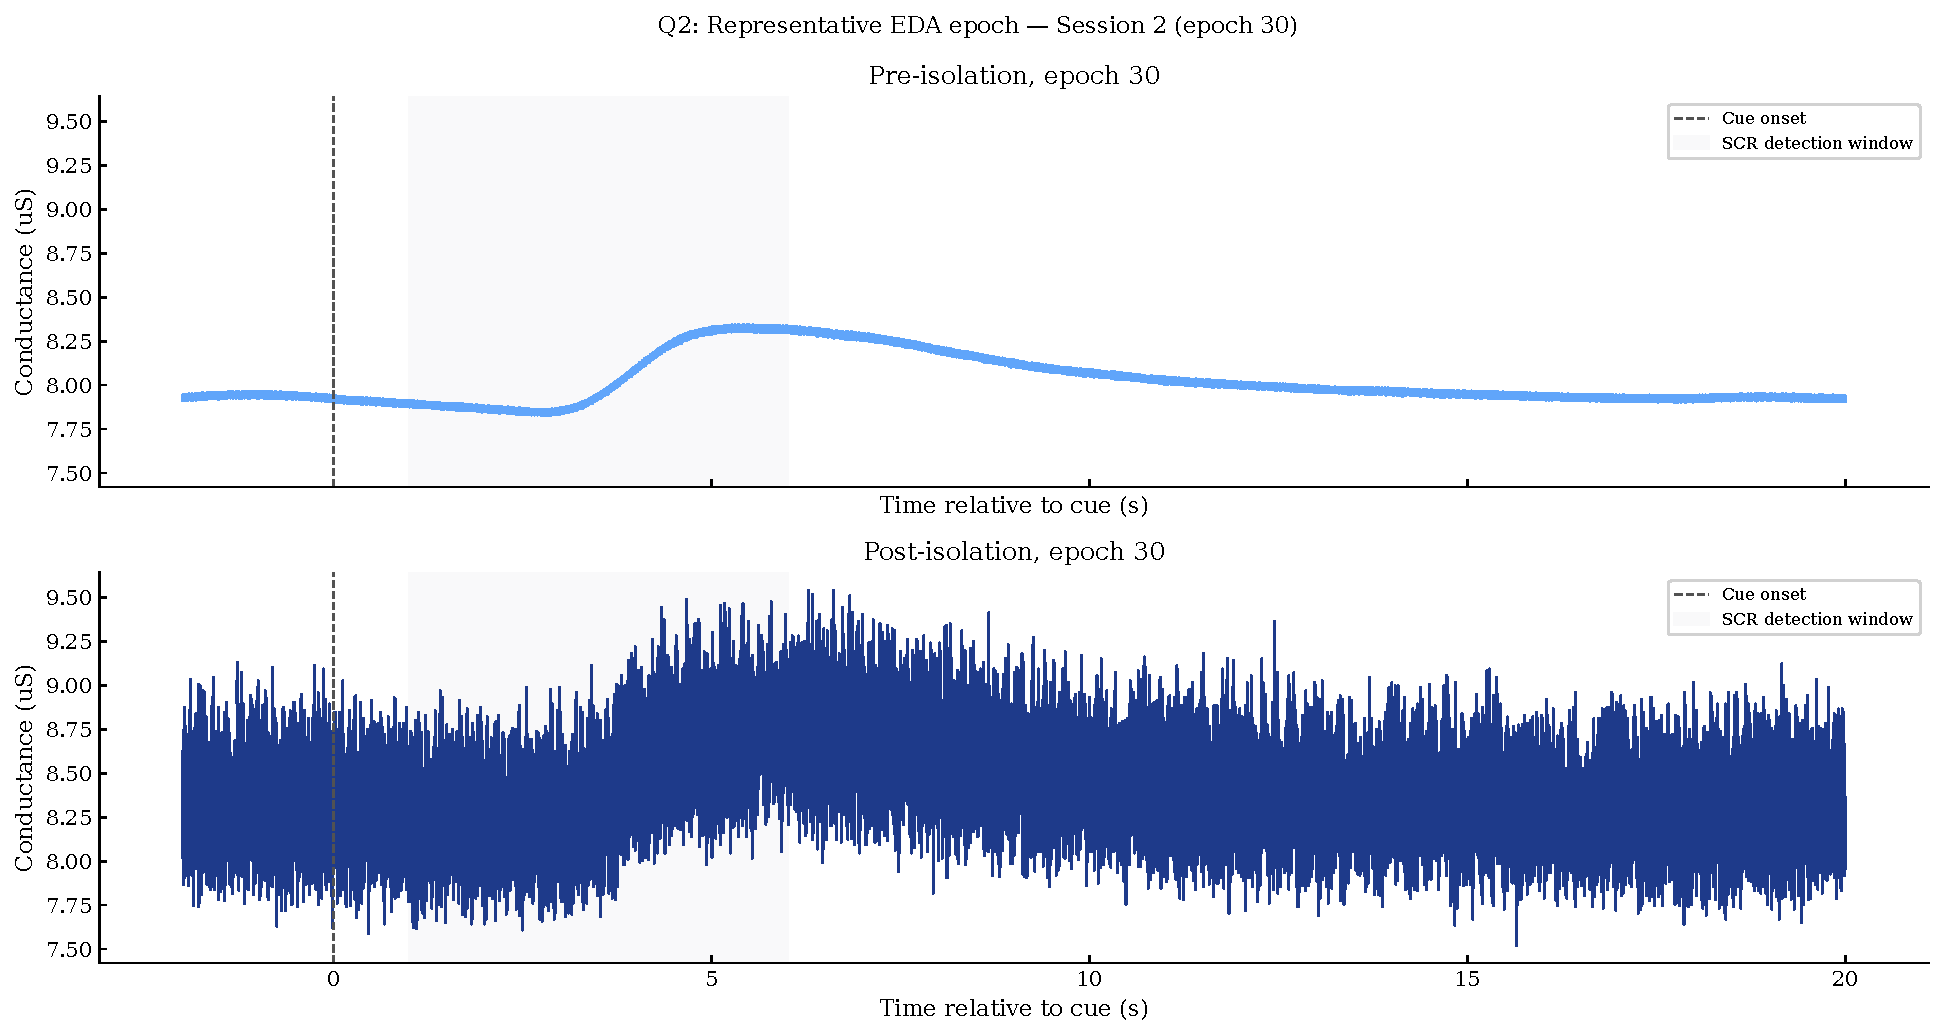
\includegraphics[width=\textwidth]{result_figures/q2_eda_representative_epoch_pre_post.pdf}
  \caption{Representative single epoch from Session~2 (epoch \num{30} of \num{30}), shown on the pre-isolation channel (top) and post-isolation channel (bottom). Dashed vertical line marks cue onset. Shaded region marks the \SIrange{1}{6}{\second} \gls{scr} detection window.}
  \label{fig:q2-eda-representative}
\end{figure}

The post-isolation \gls{scl} measured across the \num{30} epochs of Session~2 was $\num{7.714} \pm \num{0.398}$\,\si{\micro\siemens}. Mean \gls{scr} amplitude was $\num{0.588} \pm \num{0.158}$\,\si{\micro\siemens}, and rise time was $\num{3.751} \pm \num{0.776}$\,\si{\second}. Detection rate was \SI{100}{\percent} (\num{30}/\num{30} epochs). $\sigma_{\text{local}}$ describes within-epoch noise variability over the pre-cue window (Section~\ref{sec:eda_processing}). For Session~2, $\sigma_{\text{local}}$ was $\num{0.193} \pm \num{0.021}$\,\si{\micro\siemens}. Figure~\ref{fig:q2-eda-overlay} shows the signal across these epochs.

\begin{figure}[!htbp]
  \centering
  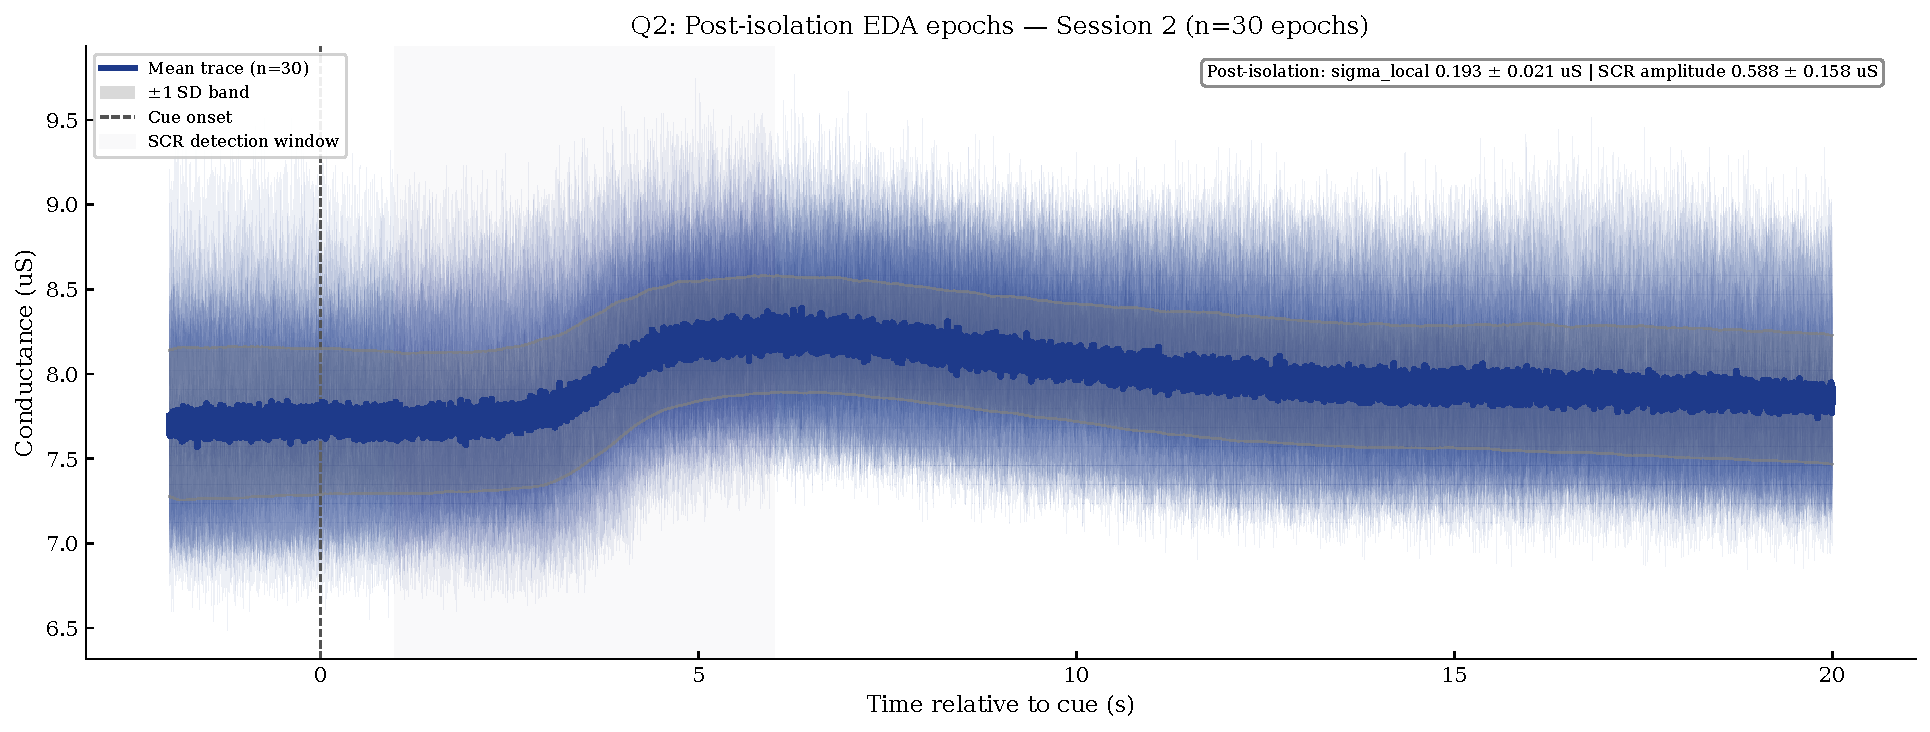
\includegraphics[width=\textwidth]{result_figures/q2_eda_overlay_post.pdf}
  \caption{Post-isolation \gls{eda} signal across the \num{30} epochs of Session~2. The solid line shows the across-epoch mean, and the grey band shows $\pm 1$ SD across epochs. $\sigma_{\text{local}}$ and \gls{scr} amplitude are annotated. Light blue traces show individual epochs.}
  \label{fig:q2-eda-overlay}
\end{figure}

$\sigma_{\text{session}}$ describes long-timescale variability across the stabilization recording (Section~\ref{sec:eda_processing}). For Session~2, $\sigma_{\text{session}}$ was \SI{0.549}{\micro\siemens}. \gls{snr}$_{\text{circuit}}$ was \SI{0.60}{\decibel} (using $\sigma_{\text{session}}$), and \gls{snr}$_{\text{local}}$ was \SI{9.66}{\decibel} (using $\sigma_{\text{local}}$). Figure~\ref{fig:q2-eda-psd} shows the post-isolation \gls{psd}. Table~\ref{tab:q2-eda-metrics} summarizes the per-epoch metrics.

\begin{figure}[!htbp]
  \centering
  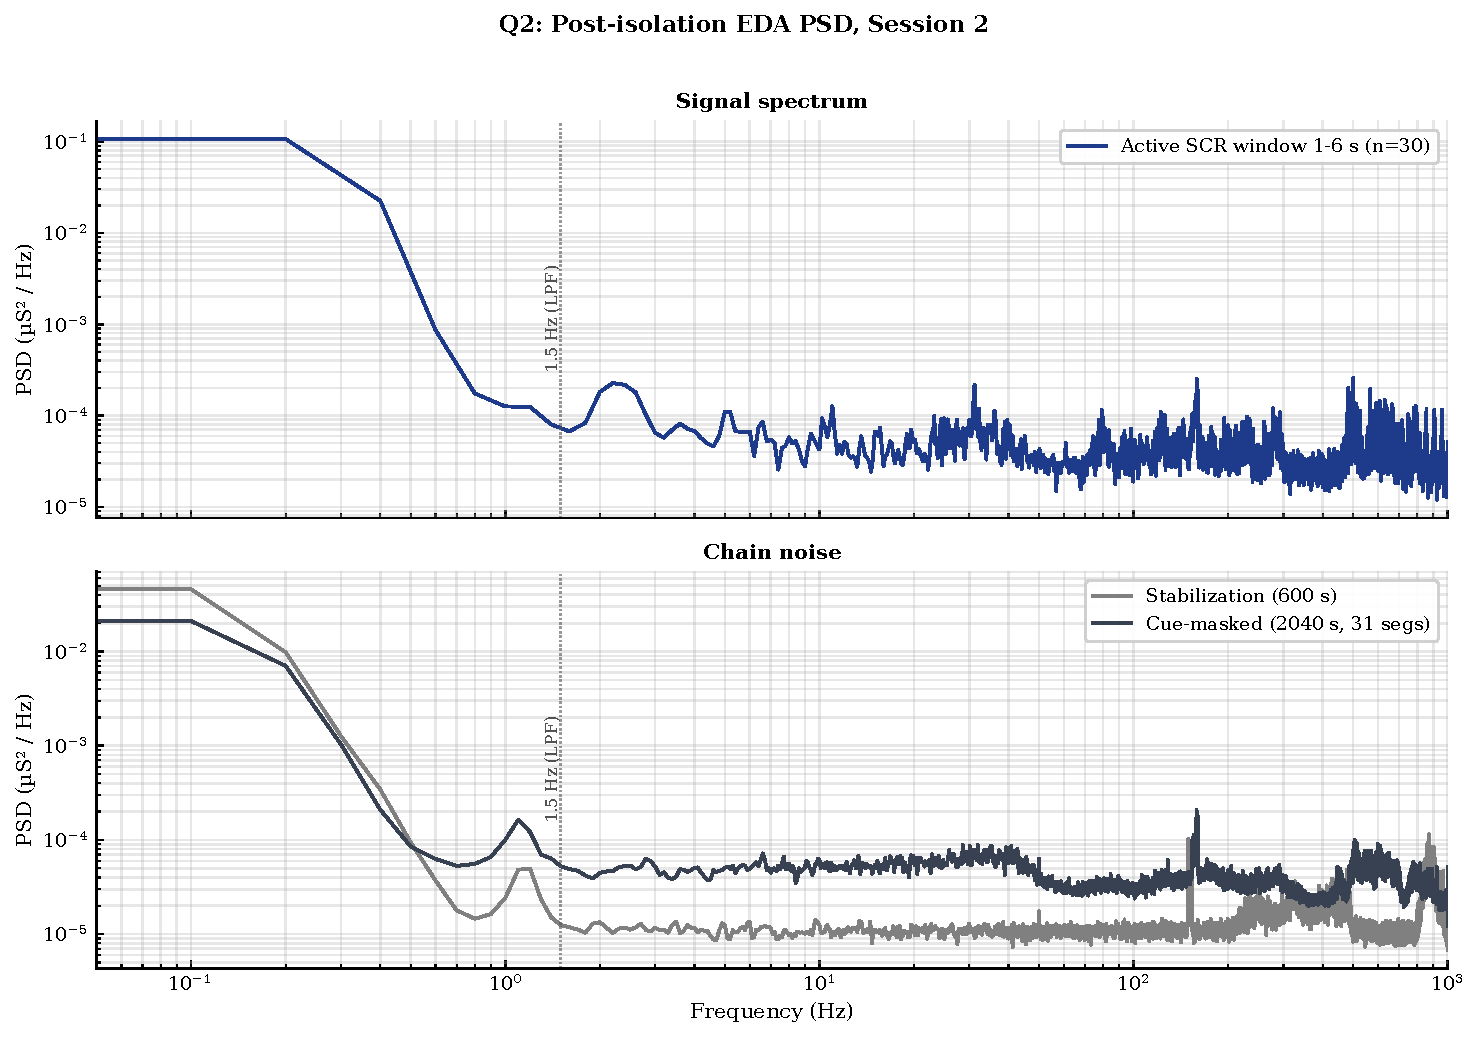
\includegraphics[width=\textwidth]{result_figures/q2_eda_psd.pdf}
  \caption{Post-isolation \gls{eda} \gls{psd}, Session~2. Top panel: signal spectrum from the active \SIrange{1}{6}{\second} \gls{scr} window. Bottom panel: chain-noise spectrum from the stabilization and cue-masked windows. The vertical line marks the analog \gls{lpf} cutoff at \SI{1.5}{\hertz}.}
  \label{fig:q2-eda-psd}
\end{figure}

\begin{table}[!htbp]
  \centering
  \caption{Post-isolation \gls{eda} metrics, Session~2 ($n = \num{30}$ epochs, all detected). Mean $\pm$ SD across epochs (or detected epochs where indicated).}
  \label{tab:q2-eda-metrics}
  \begin{tabular}{l c l}
    \toprule
    \textbf{Metric} & \textbf{Value} & \textbf{Unit} \\
    \midrule
    \gls{scl}                                                  & $\num{7.714} \pm \num{0.398}$ & \si{\micro\siemens} \\
    $\sigma_{\text{session}}$                                  & \num{0.549}                   & \si{\micro\siemens} \\
    $\sigma_{\text{local}}$                                    & $\num{0.193} \pm \num{0.021}$ & \si{\micro\siemens} \\
    \addlinespace
    \gls{scr} amplitude\textsuperscript{*}                     & $\num{0.588} \pm \num{0.158}$ & \si{\micro\siemens} \\
    Rise time\textsuperscript{*}                               & $\num{3.751} \pm \num{0.776}$ & \si{\second} \\
    Detection rate                                             & \num{100.0}                   & \si{\percent} \\
    \addlinespace
    \gls{snr}$_{\text{circuit}}$\textsuperscript{\textdagger}  & \num{0.60}                    & \si{\decibel} \\
    \gls{snr}$_{\text{local}}$\textsuperscript{\textdaggerdbl} & \num{9.66}                    & \si{\decibel} \\
    \bottomrule
  \end{tabular}
  \\[0.5em]
  {\footnotesize \textsuperscript{*}Computed over detected epochs only. \textsuperscript{\textdagger}\gls{snr}$_{\text{circuit}} = 20\log_{10}(\text{mean SCR amplitude} / \sigma_{\text{session}})$. \textsuperscript{\textdaggerdbl}\gls{snr}$_{\text{local}} = 20\log_{10}(\text{mean SCR amplitude} / \text{mean }\sigma_{\text{local}})$.}
\end{table}
 
 
% Framing claim (locked): The isolation stage preserves EMG and EDA signal
% amplitude and waveform morphology, with quantified added noise. Pearson r
% per epoch and amplitude preservation in dB report the preservation
% quantitatively for both channels.
%
% Cross-references:
%   Methods metric definitions: \autoref{sec:methods-q3-isolation}
%   Per-channel post-isolation characterization: §4.1.1, §4.1.2.
%
% Discussion (DO NOT include here):
%   σ_iso noise model (Thread Q3.1): §5.1.
%   Two-SNR-definitions asymmetry (Thread Q3.4): §5.5.
%   EMG amplitude preservation noise inflation correction (Thread Q3.2): §5.5.
%   EDA Pearson r distributional shape / 4-of-30 low-r outliers (Thread Q3.3): §5.5.
\FloatBarrier
 
\subsection{Q3 - Isolation Stage Characterization}
\label{sec:results-q3}

The post-isolation \gls{emg} characterization is reported in Section~\ref{sec:results-q1}. This section reports the pre- versus post-isolation comparison from the same Session~1 data ($n = \num{119}$ contamination-filtered epochs). Amplitude preservation across the isolation stage was $+\SI{2.56}{\decibel}$, and the per-epoch Pearson $r$ between the gain-corrected pre- and post-isolation channels was $\num{0.542} \pm \num{0.079}$. \gls{snr} was $\num{10.80} \pm \num{2.63}$\,\si{\decibel} pre-isolation and $\num{3.32} \pm \num{1.34}$\,\si{\decibel} post-isolation, a drop of $\SI{-7.48}{\decibel}$ (computed as post minus pre). Figure~\ref{fig:q3-emg-preservation} shows the time-domain and frequency-domain comparison for both channels, and the per-epoch Pearson $r$ distribution is shown in the left panel of Figure~\ref{fig:q3-pearson-r}.

\begin{figure}[!htbp]
  \centering
  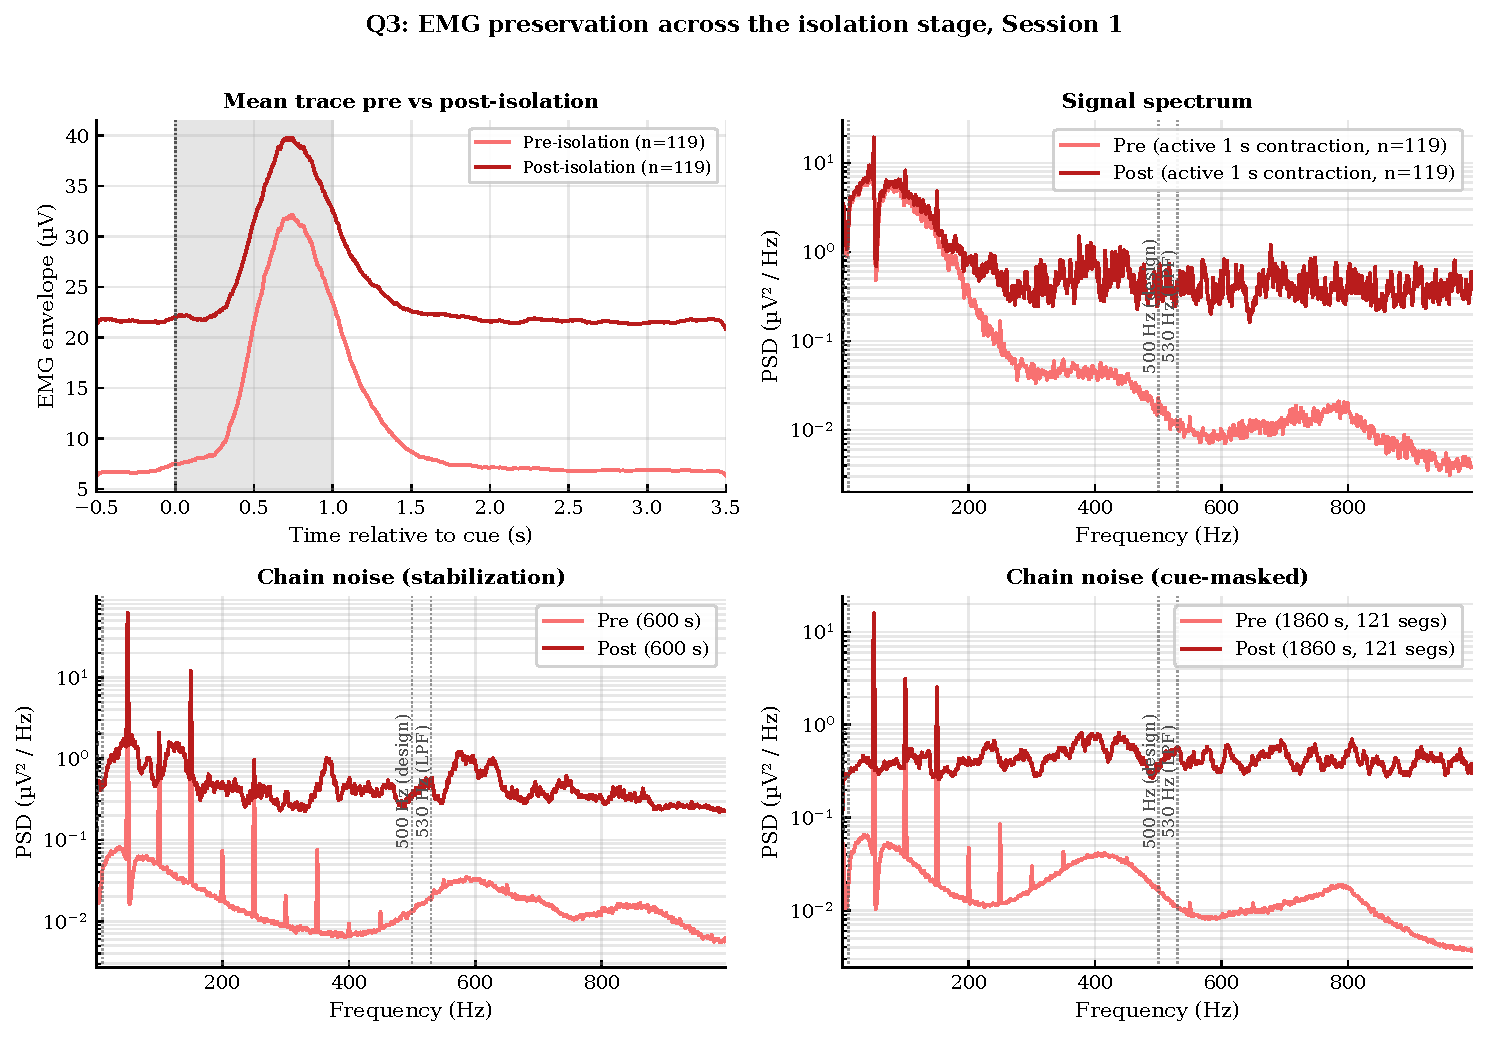
\includegraphics[width=\textwidth]{result_figures/q3_emg_preservation.pdf}
  \caption{\gls{emg} preservation across the isolation stage, Session~1. Top-left panel: across-epoch envelope mean. Top-right panel: signal spectrum. Bottom-left panel: chain-noise spectrum from the stabilization windows. Bottom-right panel: chain-noise spectrum from the cue-masked windows. Each \gls{psd} panel overlays the pre-isolation (light red) and post-isolation (dark red) channels and marks the analog \gls{hpf} cutoff at \SI{10}{\hertz}, the design bandwidth at \SI{500}{\hertz}, and the analog \gls{lpf} cutoff at \SI{530}{\hertz}.}
  \label{fig:q3-emg-preservation}
\end{figure}

The post-isolation \gls{eda} characterization is reported in Section~\ref{sec:results-q2}. This section reports the pre- versus post-isolation comparison from the same Session~2 data ($n = \num{30}$ epochs). Amplitude preservation across the isolation stage was $+\SI{1.23}{\decibel}$, and the per-epoch Pearson $r$ was $\num{0.713} \pm \num{0.162}$. \gls{scr} detection rate was \SI{100}{\percent} on both channels. \gls{snr}$_{\text{circuit}}$ was \SI{0.28}{\decibel} pre-isolation and \SI{0.60}{\decibel} post-isolation, a change of $+\SI{0.32}{\decibel}$. \gls{snr}$_{\text{local}}$ was \SI{32.63}{\decibel} pre-isolation and \SI{9.66}{\decibel} post-isolation, a drop of $\SI{-22.97}{\decibel}$. Figure~\ref{fig:q3-eda-preservation} shows the time-domain and frequency-domain comparison for both channels, and the per-epoch Pearson $r$ distribution is shown in the right panel of Figure~\ref{fig:q3-pearson-r}. Tables~\ref{tab:q3-isolation-state} and~\ref{tab:q3-isolation-change} summarize the state and change metrics for both modalities.

\begin{figure}[!htbp]
  \centering
  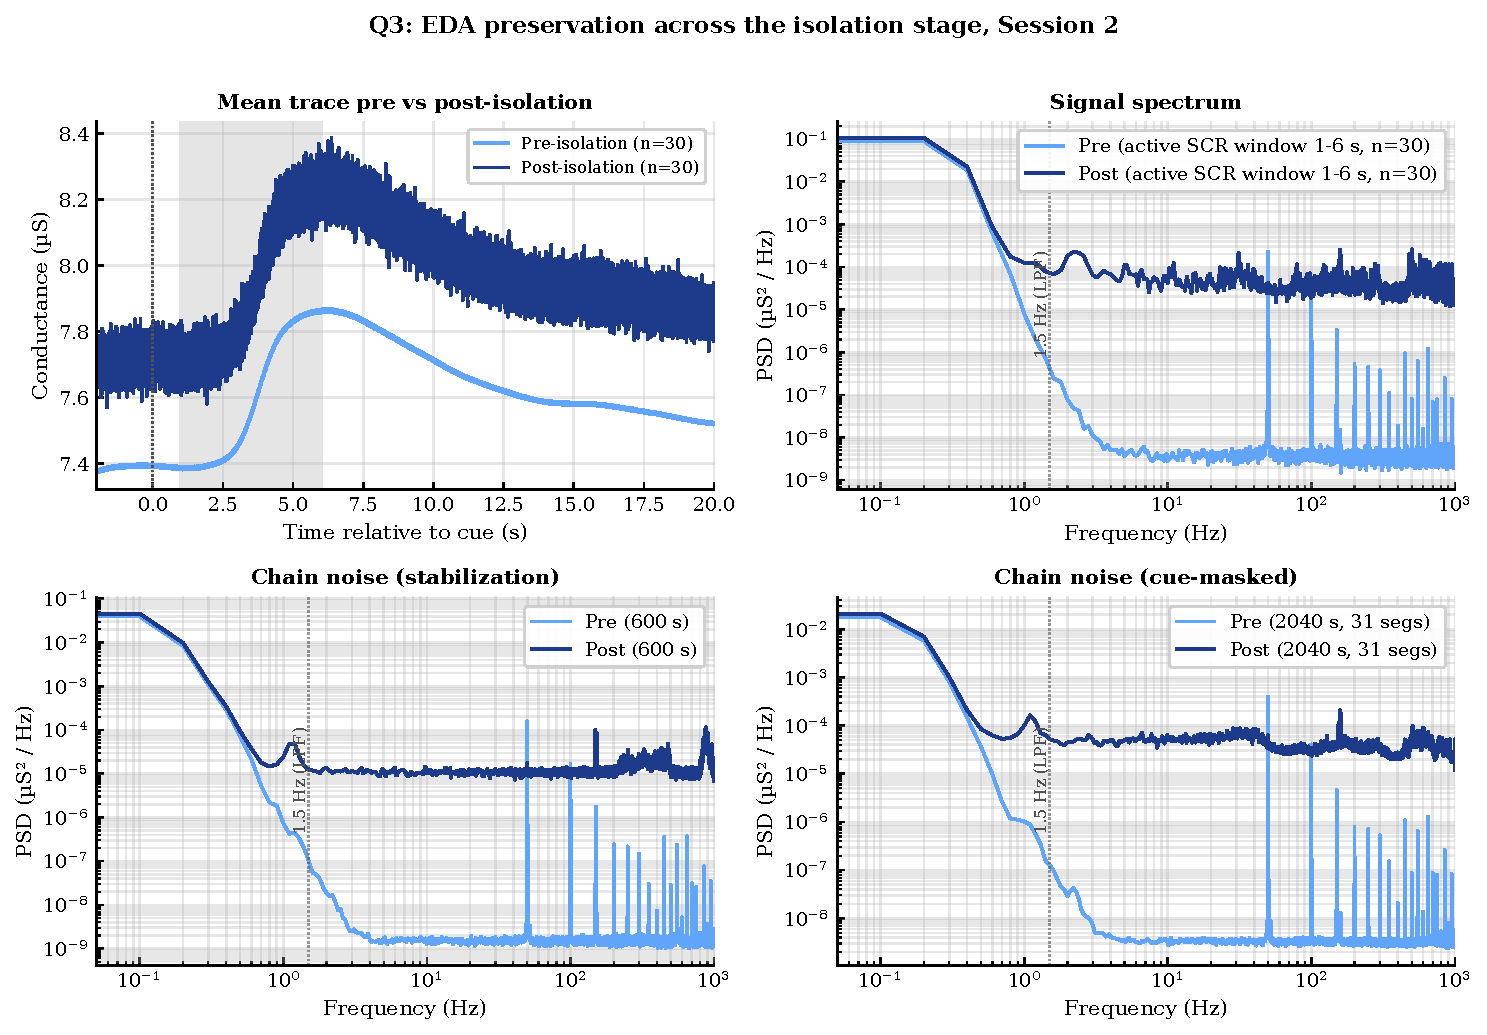
\includegraphics[width=\textwidth]{result_figures/q3_eda_preservation.pdf}
  \caption{\gls{eda} preservation across the isolation stage, Session~2. Top-left panel: across-epoch mean conductance. Top-right panel: signal spectrum. Bottom-left panel: chain-noise spectrum from the stabilization windows. Bottom-right panel: chain-noise spectrum from the cue-masked stabilization windows. Each \gls{psd} panel overlays the pre-isolation (light blue) and post-isolation (dark blue) channels and marks the analog \gls{lpf} cutoff at \SI{1.5}{\hertz}.}
  \label{fig:q3-eda-preservation}
\end{figure}

\begin{figure}[!htbp]
  \centering
  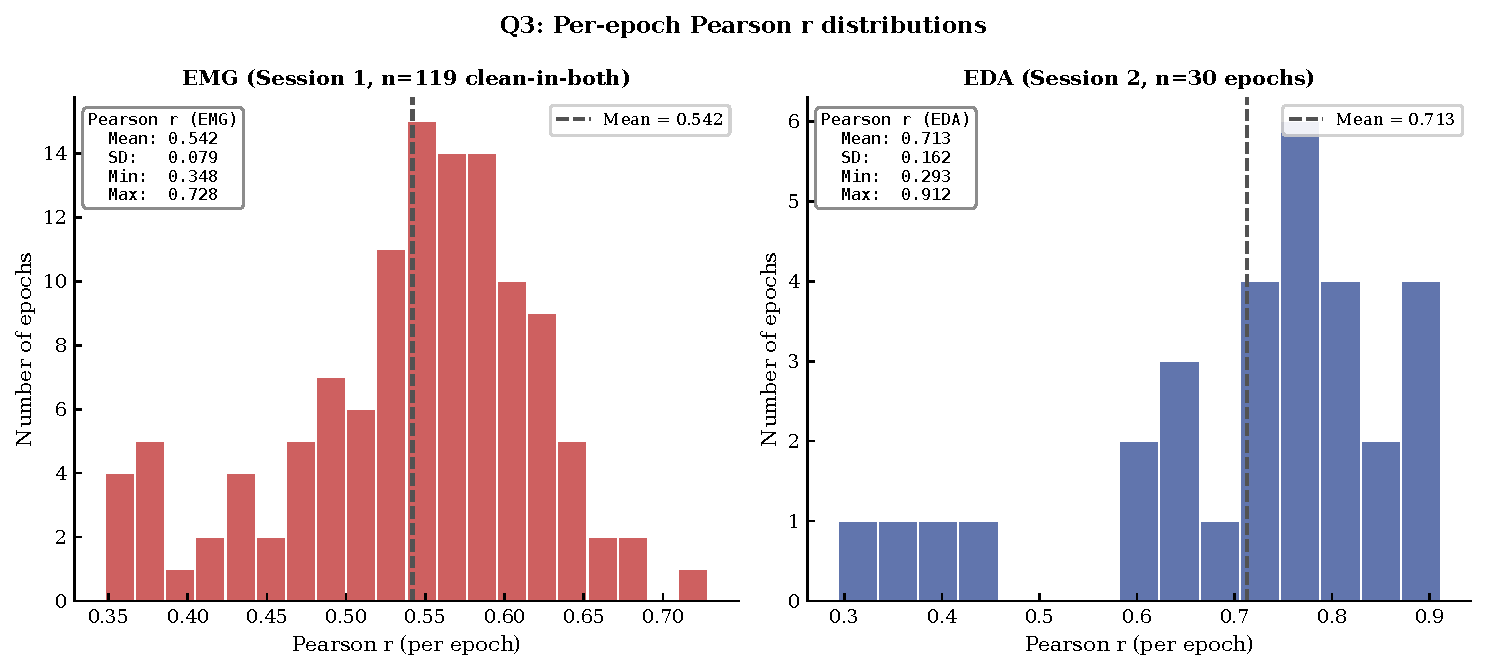
\includegraphics[width=\textwidth]{result_figures/q3_isolation_pearson_r_histograms.pdf}
  \caption{Distribution of per-epoch Pearson $r$ between pre- and post-isolation channels. Left: \gls{emg} (Session~1, $n = \num{119}$). Right: \gls{eda} (Session~2, $n = \num{30}$). Each panel marks the distribution mean and lists summary statistics.}
  \label{fig:q3-pearson-r}
\end{figure}

\begin{table}[!htbp]
  \centering
  \caption{Pre- and post-isolation state metrics for both modalities.}
  \label{tab:q3-isolation-state}
  \begin{tabular}{l c c l}
    \toprule
    \textbf{Metric} & \textbf{Pre} & \textbf{Post} & \textbf{Unit} \\
    \midrule
    \multicolumn{4}{l}{\textit{\gls{emg} (Session~1, $n = \num{119}$)}} \\
    \gls{snr}                    & $\num{10.80} \pm \num{2.63}$ & $\num{3.32} \pm \num{1.34}$ & \si{\decibel} \\
    \addlinespace
    \multicolumn{4}{l}{\textit{\gls{eda} (Session~2, $n = \num{30}$)}} \\
    \gls{snr}$_{\text{circuit}}$ & $\num{0.28}$  & $\num{0.60}$ & \si{\decibel} \\
    \gls{snr}$_{\text{local}}$   & $\num{32.63}$ & $\num{9.66}$ & \si{\decibel} \\
    \gls{scr} detection rate     & $\num{100.0}$ & $\num{100.0}$ & \si{\percent} \\
    \bottomrule
  \end{tabular}
\end{table}

\begin{table}[!htbp]
  \centering
  \caption{Isolation stage change metrics for both modalities. Amplitude preservation reported in dB as $20\log_{10}(\text{post} / \text{pre})$. Pearson $r$ reported as mean $\pm$ SD across per-epoch values for EMG and as median across per-epoch values for EDA. \gls{snr} drop computed as post minus pre.}
  \label{tab:q3-isolation-change}
  \begin{tabular}{l c l}
    \toprule
    \textbf{Metric} & \textbf{Value} & \textbf{Unit} \\
    \midrule
    \multicolumn{3}{l}{\textit{\gls{emg} (Session~1, $n = \num{119}$)}} \\
    Amplitude preservation        & $+\num{2.56}$                 & \si{\decibel} \\
    Pearson $r$ per epoch         & $\num{0.542} \pm \num{0.079}$ & --- \\
    \gls{snr} drop                & $-\num{7.48}$                 & \si{\decibel} \\
    \addlinespace
    \multicolumn{3}{l}{\textit{\gls{eda} (Session~2, $n = \num{30}$)}} \\
    Amplitude preservation               & $+\num{1.23}$                 & \si{\decibel} \\
    Pearson $r$ per epoch                & $\num{0.713} \pm \num{0.162}$ & --- \\
    Pearson $r$ median                   & $\num{0.759}$                 & --- \\
    \gls{snr}$_{\text{circuit}}$ drop    & $+\num{0.32}$                 & \si{\decibel} \\
    \gls{snr}$_{\text{local}}$ drop      & $-\num{22.97}$                & \si{\decibel} \\
    \bottomrule
  \end{tabular}
\end{table}

% Framing claim (locked): Digital post-filtering reduces the EMG noise floor
% and increases SNR at both the pre- and post-isolation stages. The notch
% filter strongly attenuates the 50 Hz mains harmonic, but the post-isolation
% notch depth is shallower than the pre-isolation depth.
%
% Main evidence:
%   q4_emg_means_raw_vs_filtered  P1, Main-Quantitative (4-condition envelope means)
%   q4_emg_psd                    P2, Main-Quantitative (2-panel stacked:
%                                  signal spectrum + chain noise, 4 conditions per panel)
%   q4_emg_waveform_single_epoch  P3, Main-Qualitative (single epoch, pre/post × raw/filtered)
%
% Cross-references:
%   Methods filter chain definitions: \autoref{sec:methods-q4-digital}
%   Pre vs post isolation context: \autoref{sec:results-q3}
%
% Discussion (DO NOT include here):
%   In-band noise architectural limit (Thread Q3.1 continuation): §5.1.
%   Notch asymmetry as ISO broadband noise signature (Thread Q3.1): §5.1.

\FloatBarrier

\subsection{Q4 - Digital Filtering}
\label{sec:results-q4}

Figure~\ref{fig:q4-emg-waveform} shows a single contraction epoch from Session~1 across the four conditions: pre-isolation raw, pre-isolation filtered, post-isolation raw, and post-isolation filtered. The post-isolation panels show visibly more noise than the pre-isolation panels.

\begin{figure}[!htbp]
  \centering
  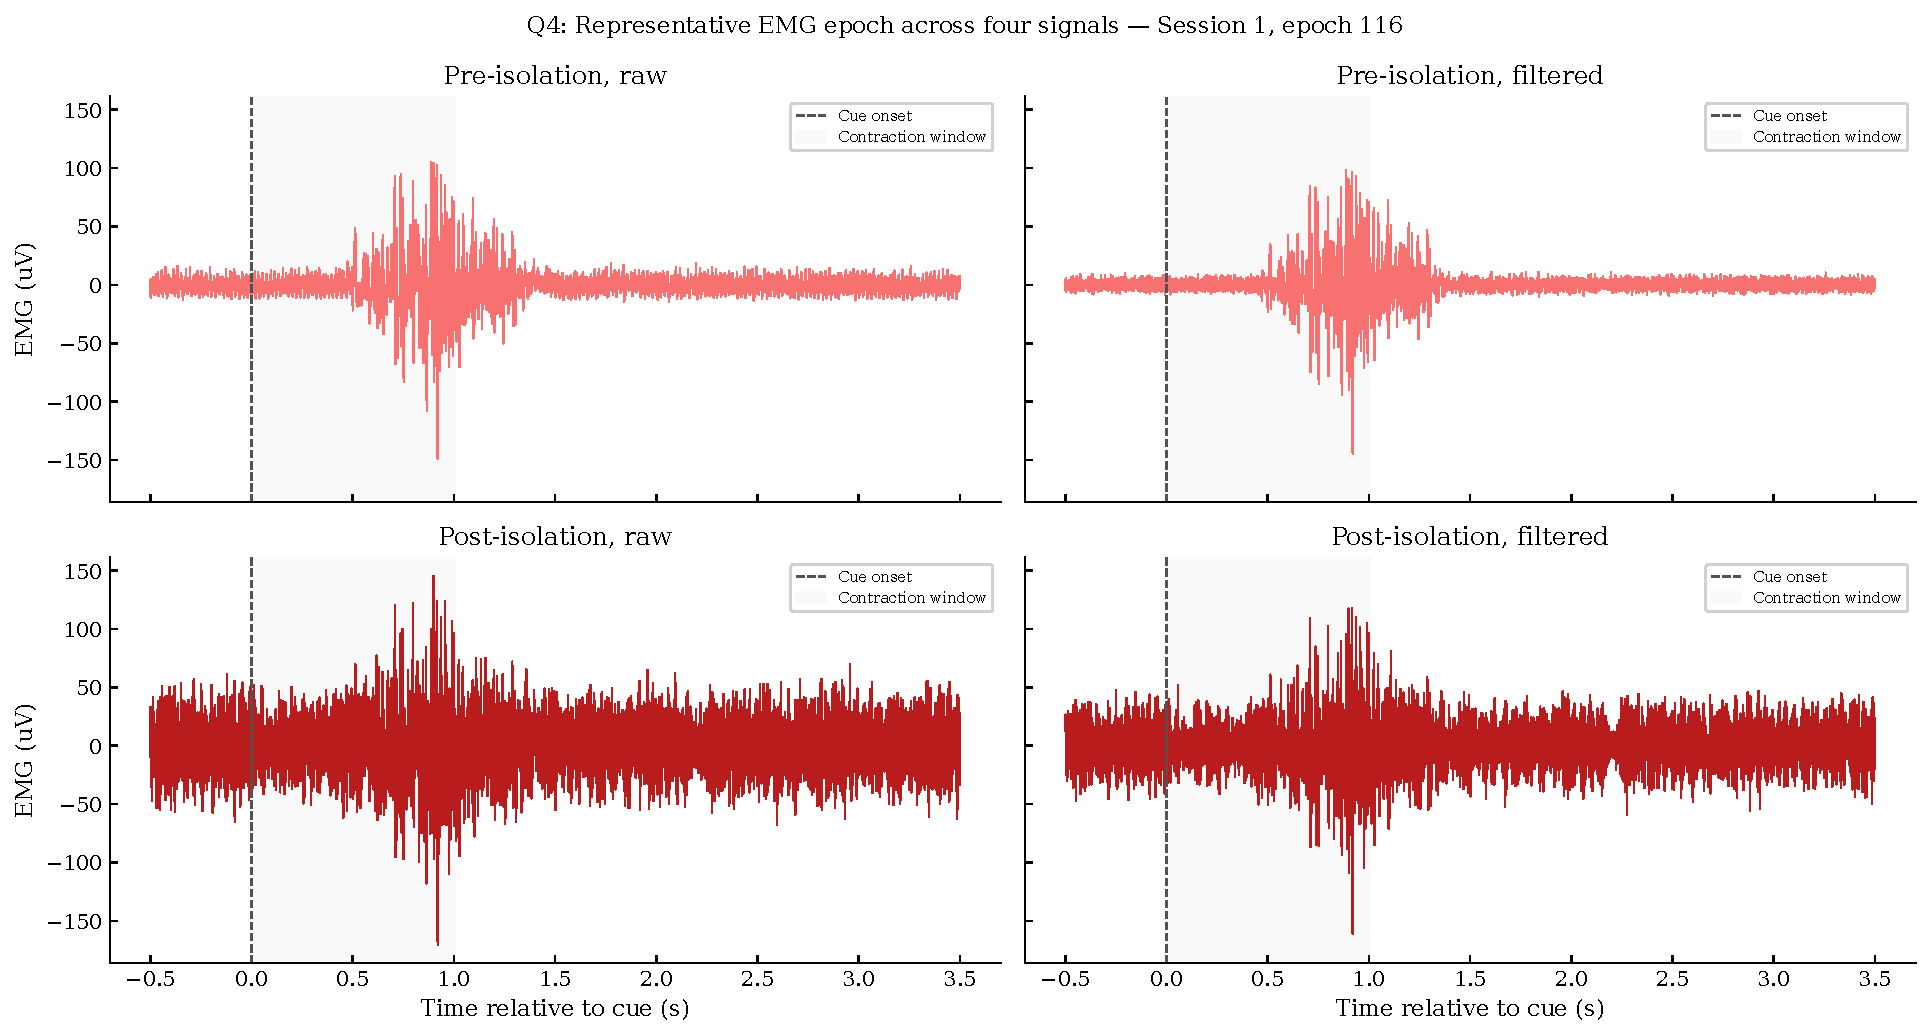
\includegraphics[width=\textwidth]{result_figures/q4_emg_waveform_single_epoch.pdf}
  \caption{Single-epoch \gls{emg} waveform comparison, Session~1. Top row: pre-isolation raw (left) and pre-isolation filtered (right). Bottom row: post-isolation raw (left) and post-isolation filtered (right). Same epoch index across panels. Dashed vertical line marks cue onset. Shaded region marks the \SI{1.0}{\second} contraction window.}
  \label{fig:q4-emg-waveform}
\end{figure}

The pre-raw and post-raw scalar metrics match those reported in Section~\ref{sec:results-q3}. This section adds the filtered conditions. Figure~\ref{fig:q4-emg-means} shows the across-epoch envelope mean for all four conditions. In the post-isolation chain, the noise floor dropped from $\num{21.70} \pm \num{0.99}$\,\si{\micro\volt} (raw) to $\num{14.12} \pm \num{2.82}$\,\si{\micro\volt} (filtered), contraction \gls{rms} dropped from $\num{32.17} \pm \num{4.98}$ to $\num{26.28} \pm \num{4.57}$\,\si{\micro\volt}, and \gls{snr} rose from $\num{3.32} \pm \num{1.34}$ to $\num{5.45} \pm \num{2.74}$\,\si{\decibel}. The pre-isolation chain showed the same direction of change. Post-filtered scalar metrics did not match pre-raw values: noise floor was \SI{14.12}{\micro\volt} versus \SI{6.84}{\micro\volt} pre-raw, and \gls{snr} was \SI{5.45}{\decibel} versus \SI{10.80}{\decibel} pre-raw. Table~\ref{tab:q4-emg-metrics} summarizes the per-condition metrics.

\begin{figure}[!htbp]
  \centering
  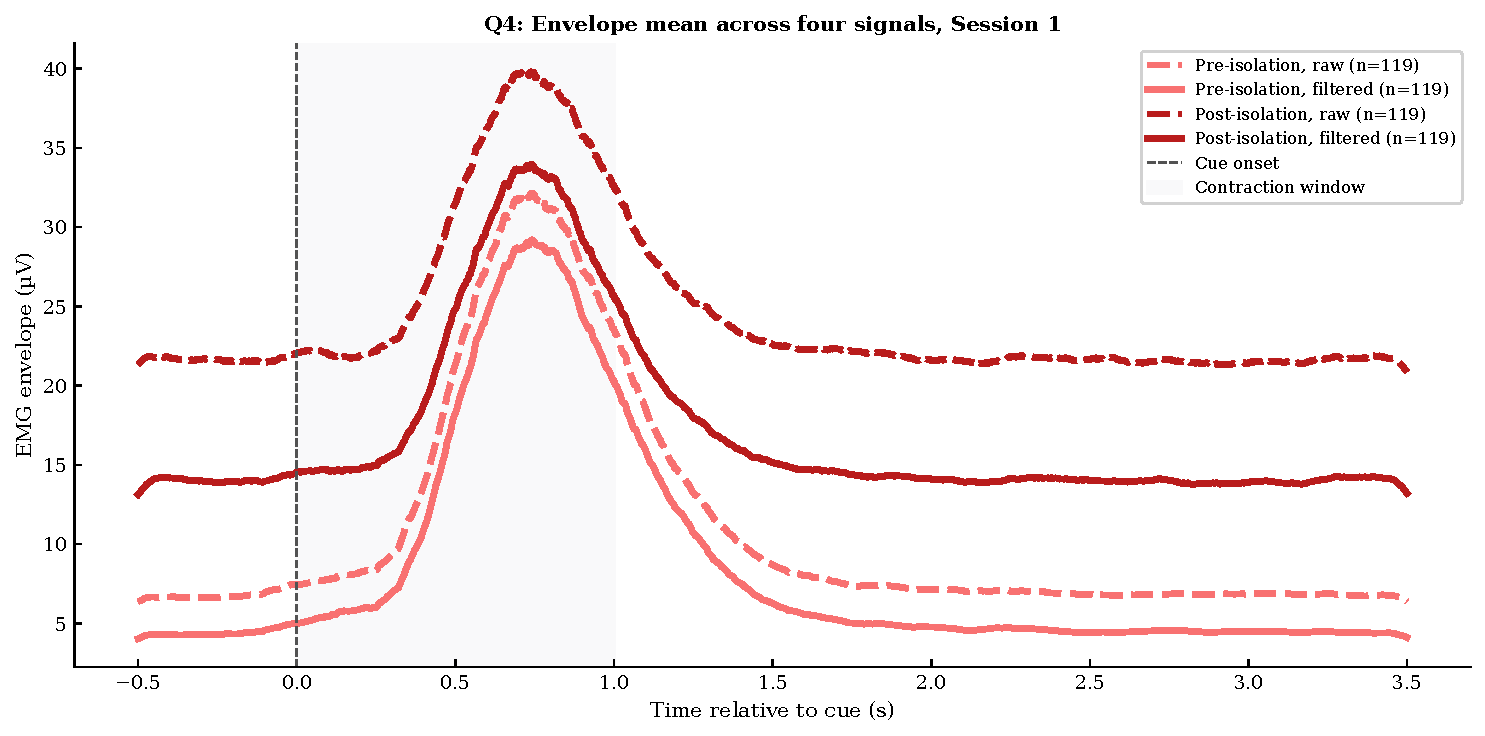
\includegraphics[width=\textwidth]{result_figures/q4_emg_means_raw_vs_filtered.pdf}
  \caption{\gls{emg} envelope mean across the four conditions of Session~1 ($n = \num{119}$): pre-raw, pre-filtered, post-raw, post-filtered. Dashed vertical line marks cue onset. Shaded region marks the \SI{1.0}{\second} contraction window.}
  \label{fig:q4-emg-means}
\end{figure}

Figure~\ref{fig:q4-emg-psd-four} shows the \gls{psd} for each of the four conditions. The notch filter visibly suppresses the \SI{50}{\hertz} mains harmonic in both filtered conditions. Table~\ref{tab:q4-emg-metrics} reports integrated band powers at the \SI{50}{\hertz}, \SI{100}{\hertz}, and \SI{150}{\hertz} mains harmonics from the active-window signal spectrum. Integrated power at the \SI{50}{\hertz} harmonic dropped from \SI{28.69}{\micro\volt\squared} pre-raw to \SI{0.07}{\micro\volt\squared} pre-filtered, and from \SI{34.95}{\micro\volt\squared} post-raw to \SI{0.32}{\micro\volt\squared} post-filtered. Integrated power at the \SI{100}{\hertz} and \SI{150}{\hertz} harmonics was unchanged across the raw and filtered conditions. Integrated notch depth at \SI{50}{\hertz} was \SI{26.18}{\decibel} for the pre-isolation chain and \SI{20.40}{\decibel} for the post-isolation chain.

\begin{figure}[!htbp]
  \centering
  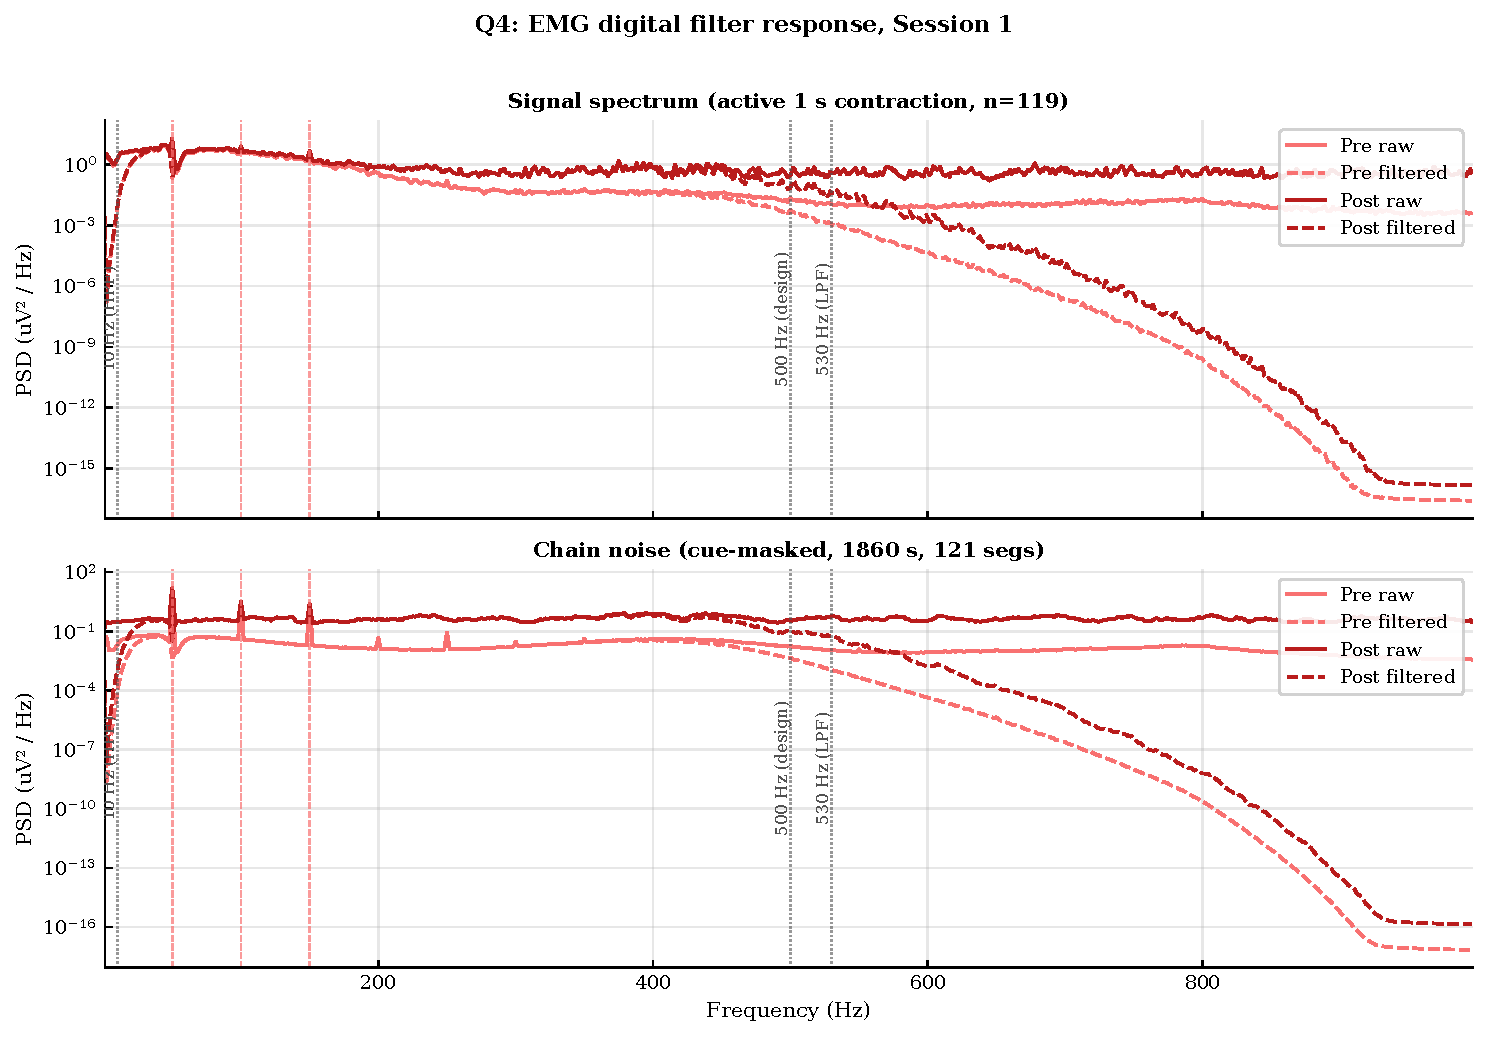
\includegraphics[width=\textwidth]{result_figures/q4_emg_psd.pdf}
  \caption{\gls{emg} \gls{psd} across the four conditions of Session~1: pre-raw, pre-filtered, post-raw, post-filtered. Top panel: signal spectrum from the active \SI{1}{\second} contraction window. Bottom panel: chain-noise spectrum from the cue-masked windows. Vertical lines mark the analog \gls{hpf} cutoff at \SI{10}{\hertz}, the design bandwidth at \SI{500}{\hertz}, and the analog \gls{lpf} cutoff at \SI{530}{\hertz}.}
  \label{fig:q4-emg-psd-four}
\end{figure}

\begin{table}[!htbp]
  \centering
  \caption{Per-condition \gls{emg} metrics, Session~1 ($n = \num{119}$). Mean $\pm$ SD across epochs. Harmonic powers computed from the active-window signal spectrum, reported as pooled Welch estimates without per-epoch SD. Notch depth at \SI{50}{\hertz} computed per chain from Equation~\ref{eq:notch_depth}. The value spans the (raw, filtered) column pair for that chain.}
  \label{tab:q4-emg-metrics}
  \begin{tabular}{l c c c c l}
    \toprule
    \textbf{Metric} & \textbf{Pre, raw} & \textbf{Pre, filt.} & \textbf{Post, raw} & \textbf{Post, filt.} & \textbf{Unit} \\
    \midrule
    Noise floor          & $\num{6.84}  \pm \num{1.82}$ & $\num{4.48}  \pm \num{1.16}$ & $\num{21.70} \pm \num{0.99}$ & $\num{14.12} \pm \num{2.82}$ & \si{\micro\volt} \\
    Contraction \gls{rms} & $\num{23.96} \pm \num{6.44}$ & $\num{21.51} \pm \num{6.21}$ & $\num{32.17} \pm \num{4.98}$ & $\num{26.28} \pm \num{4.57}$ & \si{\micro\volt} \\
    \gls{snr}             & $\num{10.80} \pm \num{2.63}$ & $\num{13.43} \pm \num{2.74}$ & $\num{3.32}  \pm \num{1.34}$ & $\num{5.45}  \pm \num{2.74}$ & \si{\decibel} \\
    \addlinespace
    Harmonic power, \SI{50}{\hertz}  & \num{28.69} & \num{0.07} & \num{34.95} & \num{0.32} & \si{\micro\volt\squared} \\
    Harmonic power, \SI{100}{\hertz} & \num{4.11}  & \num{4.09} & \num{4.58}  & \num{4.56} & \si{\micro\volt\squared} \\
    Harmonic power, \SI{150}{\hertz} & \num{5.24}  & \num{5.23} & \num{6.54}  & \num{6.53} & \si{\micro\volt\squared} \\
    \addlinespace
    Notch depth, \SI{50}{\hertz} & \multicolumn{2}{c}{\num{26.18}} & \multicolumn{2}{c}{\num{20.40}} & \si{\decibel} \\
    \bottomrule
  \end{tabular}
\end{table}

\FloatBarrier

 
% =============================================================================
% 4.2 Cross-Contamination Assessment (umbrella for Q5, Q5b, Q6, Q6b)
%
% Two directions of potential interference (EMG into EDA, EDA into EMG).
% Q5/Q6 test contamination at each modality's stimulus cues. Q5b/Q6b extend
% each into a coupling test at the OTHER modality's cues.
% =============================================================================
 
\section{Cross-Contamination Assessment}
\label{sec:results-crosscontamination}

This section reports the cross-modality contamination assessment during simultaneous \gls{emg} and \gls{eda} acquisition. Two directions of potential interference are tested: \gls{emg} contamination of the \gls{eda} signal and \gls{eda} contamination of the \gls{emg} signal. For each direction, the affected modality is analyzed time-locked to its own stimulus cues. A bystander analysis, based on the cues of the other modality, extends each pair. The data are drawn from Sessions~3 to~5.

% Section opener for §4.2: introduce the cross-modality contamination
% assessment, the two directions tested (EMG → EDA, EDA → EMG), the
% time-locked vs bystander analysis split, and the data source
% (Sessions 3 to 5). One paragraph, ~5 sentences.
 
 
% Framing claim (V2 locked): SCL is consistently elevated by approximately
% +0.4 µS in the Combined block relative to EDA-only across all three
% sessions. SCR amplitude is reduced in Combined relative to EDA-only at
% the pooled level, but the per-session breakdown shows this pattern
% reverses in one of three sessions. Detection rate is at ceiling across
% all conditions. Low-frequency PSD shows elevation in the Combined block
% concentrated in the 0.3-1.0 Hz band.
%
%
% Cross-references:
%   Methods metric definitions: \autoref{sec:methods-q5}
%   Q5b time-locked deviation at first EMG cue: \autoref{sec:results-q5b}
%   Per-session SCL/SCR breakdown: \autoref{sec:results-q7}
%   S2 reference characterization: \autoref{sec:results-q2}
%
% Discussion (DO NOT include here):
%   SCR amplitude reproducibility issue (Thread Q5.1): §5.5.
%   PSD elevation mechanism candidates (mechanical/rail/cue-arousal/cable, Thread CrossQ.3 cue-mask): §5.5.
%   Q5 PSD spike pattern at 10-50 Hz harmonic sub-locations (Thread Q5.2): §5.5.
%   Q5 P1 dip cross-references Q5b (Thread Q5.3): §5.5.
%
% Reporting flag (write-time):
%   SCR amplitude paragraph must report pooled finding AND immediately disclose
%   the S4 reversal from the Q7 per-session table. Do NOT claim contamination.
%   Frame as "consistent in 2 of 3 sessions; S4 reverses the direction".
 

 
\subsection{Q5 - EMG Effect on EDA}
\label{sec:results-q5}

Figure~\ref{fig:q5-eda-means} shows the across-epoch mean conductance per condition. The Session~2 reference is characterized in Section~\ref{sec:results-q2}, and the Sessions 3 to 5 pooled values follow the convention in Section~\ref{sec:q5_emg_effect_on_eda}. A small downward deflection is visible in the Combined trace at approximately $+\SI{5}{\second}$ relative to the \gls{eda} cue, coinciding with the first \gls{emg} cue in the Combined block. Section~\ref{sec:results-q5b} reports the cue-locked analysis. \gls{scl} was $\num{7.714} \pm \num{0.398}$\,\si{\micro\siemens} for the Session~2 reference, $\num{5.923} \pm \num{1.244}$\,\si{\micro\siemens} for the EDA-only block, and $\num{6.334} \pm \num{1.382}$\,\si{\micro\siemens} for the Combined block. The EDA-only and Combined pooled means were \SI{1.79}{\micro\siemens} and \SI{1.38}{\micro\siemens} below the Session~2 reference, respectively. The per-session \gls{scl} shift (Combined minus EDA-only) was $+\num{0.332}$\,\si{\micro\siemens} for S3, $+\num{0.228}$\,\si{\micro\siemens} for S4, and $+\num{0.675}$\,\si{\micro\siemens} for S5, with a mean of $+\num{0.412} \pm \num{0.234}$\,\si{\micro\siemens} across the three sessions. Figure~\ref{fig:q5-eda-bars} shows the per-condition \gls{scl} bars.

\begin{figure}[!htbp]
  \centering
  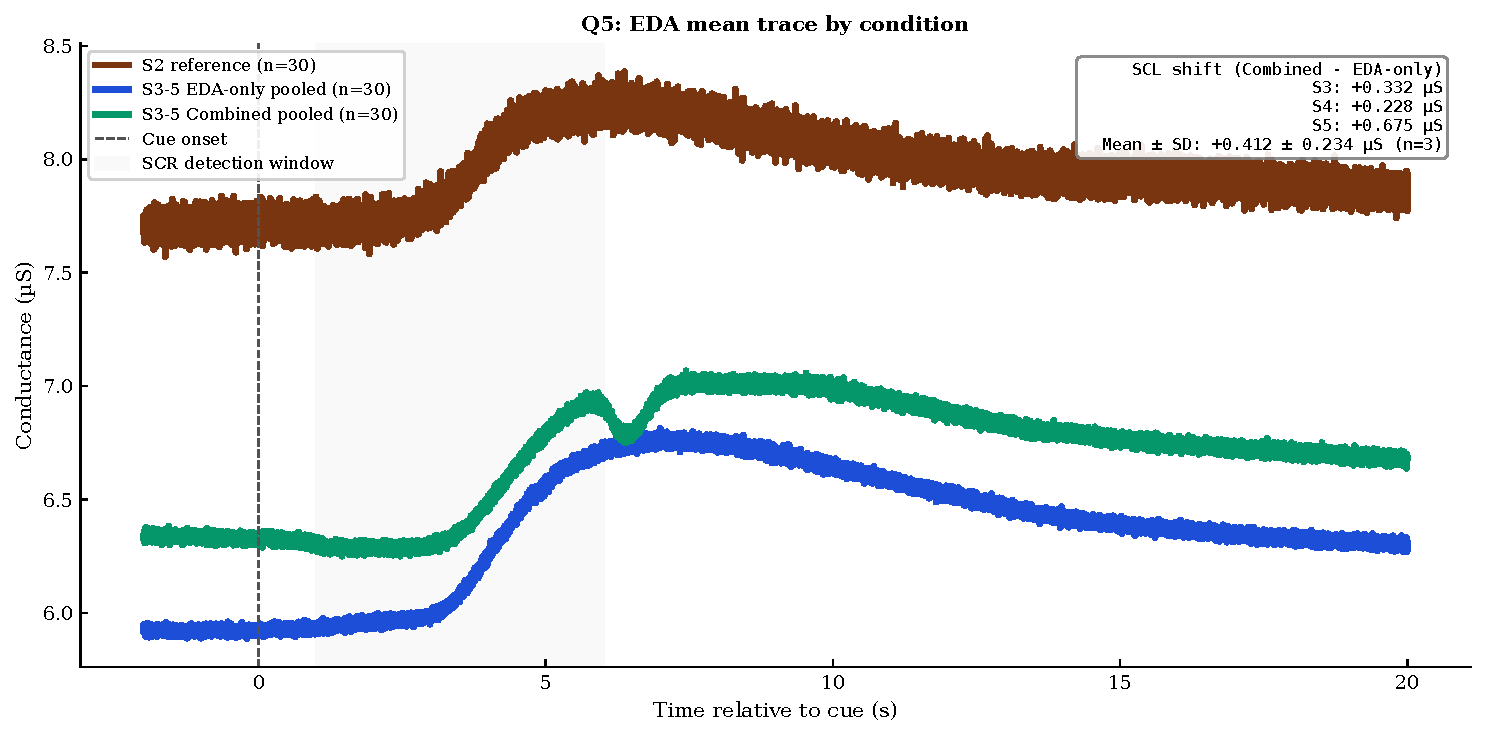
\includegraphics[width=\textwidth]{result_figures/q5_eda_means_by_condition.pdf}
  \caption{\gls{eda} mean conductance by condition: Session~2 reference ($n = \num{30}$), Sessions 3 to 5 EDA-only pooled ($n = \num{30}$), Sessions 3 to 5 Combined pooled ($n = \num{30}$). Display window $-2$ to $+20$\,\si{\second} relative to the \gls{eda} cue. Dashed vertical line marks cue onset. Shaded region marks the \SIrange{1}{6}{\second} \gls{scr} detection window. Inset reports the per-session \gls{scl} shift (Combined minus EDA-only).}
  \label{fig:q5-eda-means}
\end{figure}

\gls{scr} amplitude was $\num{0.588} \pm \num{0.158}$\,\si{\micro\siemens} for the Session~2 reference, $\num{0.800} \pm \num{0.211}$\,\si{\micro\siemens} for the EDA-only block, and $\num{0.688} \pm \num{0.180}$\,\si{\micro\siemens} for the Combined block. The Combined-block pooled mean \gls{scr} amplitude was \SI{14}{\percent} below the EDA-only pooled mean. The per-session breakdown in Section~\ref{sec:results-q7} shows S3 and S5 with lower amplitude in Combined than in EDA-only, and S4 with the opposite direction. Detection rate was \SI{100}{\percent} across all three conditions. \gls{snr}$_{\text{circuit}}$ was \SI{0.60}{\decibel} for the Session~2 reference, $\num{7.53} \pm \num{4.39}$\,\si{\decibel} for the EDA-only block, and $\num{6.19} \pm \num{6.28}$\,\si{\decibel} for the Combined block. \gls{snr}$_{\text{local}}$ was \SI{9.66}{\decibel}, $\num{25.10} \pm \num{5.44}$\,\si{\decibel}, and $\num{22.90} \pm \num{6.20}$\,\si{\decibel} across the same three conditions.

\begin{figure}[!htbp]
  \centering
  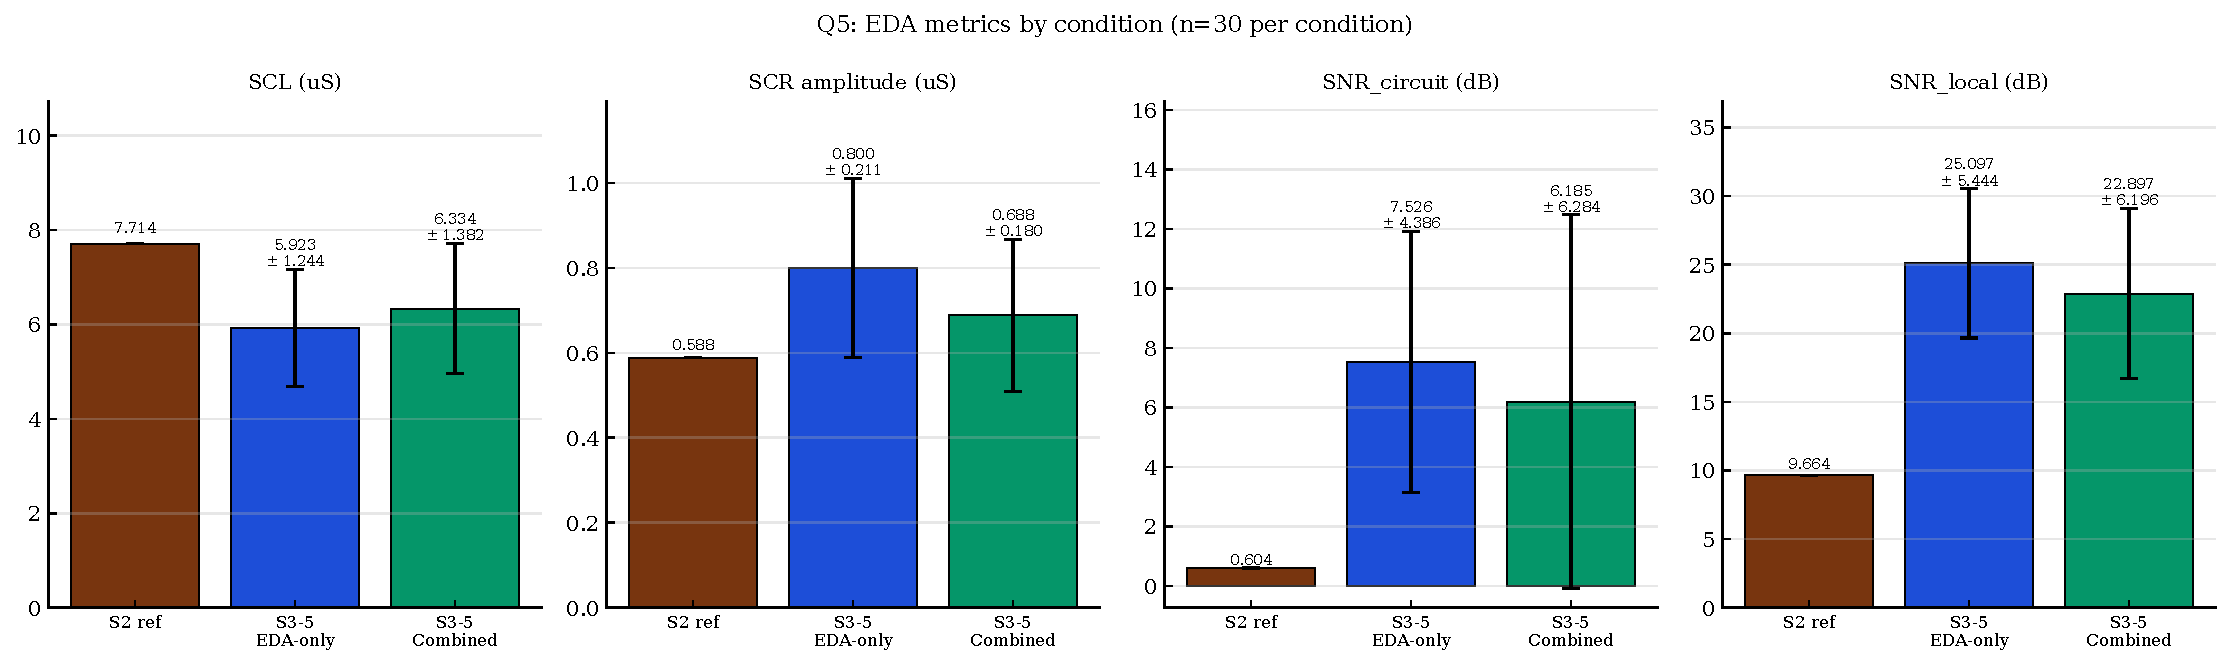
\includegraphics[width=\textwidth]{result_figures/q5_eda_metric_bars.pdf}
  \caption{\gls{eda} scalar metrics by condition: \gls{scl}, \gls{scr} amplitude, \gls{snr}$_{\text{circuit}}$, and \gls{snr}$_{\text{local}}$. Bars show the Session~2 reference value alongside the Sessions 3 to 5 EDA-only and Combined block means. \gls{scl} and \gls{scr} amplitude bars show the pooled mean across epochs ($n = \num{30}$) with $\pm 1$ SD error bars. \gls{snr}$_{\text{circuit}}$ and \gls{snr}$_{\text{local}}$ bars show the across-session mean ($n = 3$ sessions) without per-epoch SD. The Session~2 reference is a single-session value. Per-epoch SDs are reported in Section~\ref{sec:results-q2}.}
  \label{fig:q5-eda-bars}
\end{figure}

Figure~\ref{fig:q5-eda-psd} shows the \gls{eda} \gls{psd} per condition. The Combined trace exceeds the EDA-only trace across the \SIrange{0.3}{1.3}{\hertz} band and approaches the Session~2 reference level above approximately \SI{1.3}{\hertz}. Table~\ref{tab:q5-eda-metrics} summarizes the per-condition metrics.

\begin{figure}[!htbp]
  \centering
  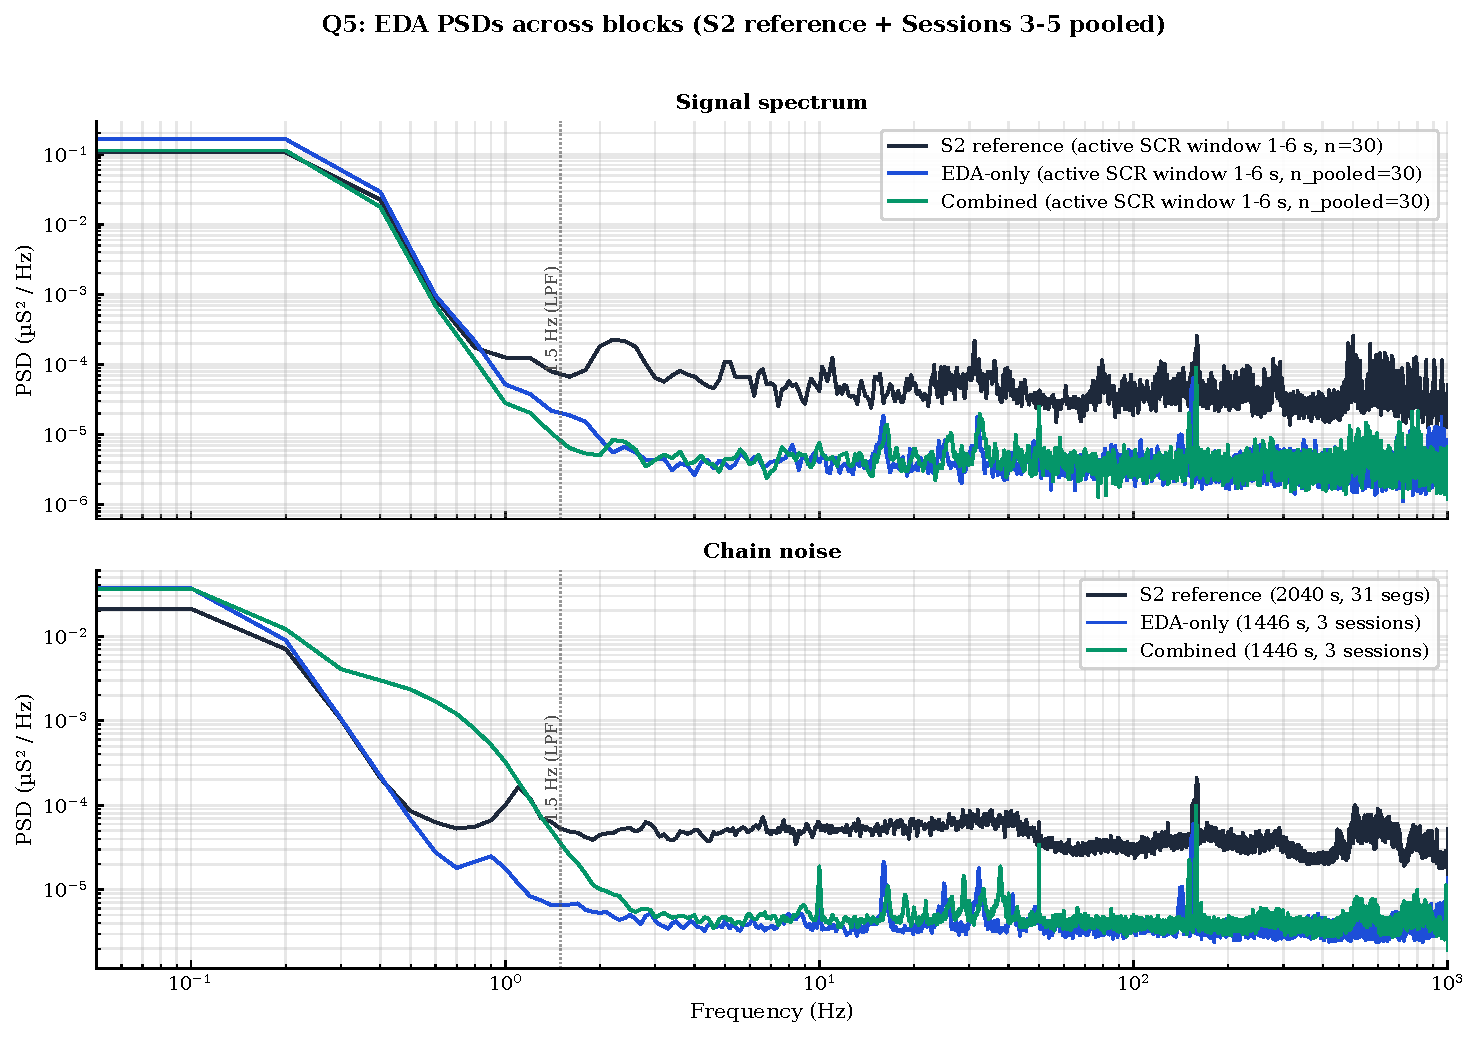
\includegraphics[width=\textwidth]{result_figures/q5_eda_psd.pdf}
  %\caption{Post-isolation \gls{eda} \gls{psd} by condition. Top panel: signal spectrum. Bottom panel: chain-noise spectrum from the cue-masked stabilization windows. Each panel overlays the Session~2 reference and the Sessions~3 to~5 EDA-only and Combined blocks pooled across epochs.}
  \caption{\gls{eda} \gls{psd} by condition. Top panel: signal spectrum. Bottom panel: chain-noise spectrum from the cue-masked windows. The vertical line marks the analog \gls{lpf} cutoff at \SI{1.5}{\hertz}.}
  \label{fig:q5-eda-psd}
\end{figure}

\begin{table}[!htbp]
  \centering
  \caption{Per-condition \gls{eda} metrics for the Session~2 reference ($n = \num{30}$) and the Sessions~3 to~5 EDA-only and Combined blocks pooled across epochs ($n = \num{30}$ each). \gls{scl} and \gls{scr} amplitude reported as pooled mean $\pm$ SD across epochs. \gls{snr}$_{\text{circuit}}$ and \gls{snr}$_{\text{local}}$ reported as across-session mean $\pm$ SD ($n = 3$ sessions), computed as session-level scalars.}
  \label{tab:q5-eda-metrics}
  \begin{tabular}{l c c c l}
    \toprule
    \textbf{Metric} & \textbf{S2 ref} & \textbf{S3-5 EDA-only} & \textbf{S3-5 Combined} & \textbf{Unit} \\
    \midrule
    \gls{scl}                    & $\num{7.714} \pm \num{0.398}$ & $\num{5.923} \pm \num{1.244}$ & $\num{6.334} \pm \num{1.382}$ & \si{\micro\siemens} \\
    \gls{scr} amplitude          & $\num{0.588} \pm \num{0.158}$ & $\num{0.800} \pm \num{0.211}$ & $\num{0.688} \pm \num{0.180}$ & \si{\micro\siemens} \\
    Detection rate               & \num{100.0}                   & \num{100.0}                   & \num{100.0}                   & \si{\percent} \\
    \addlinespace
    \gls{snr}$_{\text{circuit}}$ & \num{0.60}                    & $\num{7.53} \pm \num{4.39}$   & $\num{6.19} \pm \num{6.28}$   & \si{\decibel} \\
    \gls{snr}$_{\text{local}}$   & \num{9.66}                    & $\num{25.10} \pm \num{5.44}$  & $\num{22.90} \pm \num{6.20}$  & \si{\decibel} \\
    \bottomrule
  \end{tabular}
  \\[0.5em]
  {\footnotesize \gls{scl} shift (Combined minus EDA-only, paired by session, $n = 3$): $+\num{0.412} \pm \num{0.234}$\,\si{\micro\siemens}. Per-session: S3 $+\num{0.332}$, S4 $+\num{0.228}$, S5 $+\num{0.675}$\,\si{\micro\siemens}.}
\end{table}
 
 
% Framing claim (V2 locked, post σ_local audit): A small positive deviation in
% EDA conductance is observed time-locked to EMG cues across all three sessions,
% with latency clustering around 1.3-1.5 s post-cue. Sign convention: positive
% deviation amplitude = downward deflection from pre-cue baseline.
%
% Cross-references:
%   Methods metric definitions: \autoref{sec:methods-q5b}
%   Q5 P1 mean trace dip aligned with first EMG cue: \autoref{sec:results-q5}
%
% Discussion (DO NOT include here):
%   Mechanism candidates (mechanical/vascular coupling at palm site): §5.5.
%   Site-specificity of the coupling (palm vs biceps): §5.5 / §5.4.
%   σ_local pre/post audit and decision rationale: methodological log.
 
\subsection{Q5b - EDA Response at EMG Cues}
\label{sec:results-q5b}

This section reports the cue-locked analysis of the \gls{eda} signal at \gls{emg} cues, referenced in Section~\ref{sec:results-q5}. Figure~\ref{fig:q5b-eda-by-session} shows the \gls{eda} signal time-locked to \gls{emg} cues in the EMG-only block of Sessions 3 to 5, where no \gls{eda} stimulus was delivered. A small downward dip is visible in the \gls{eda} signal beginning shortly after each cue and resolving within approximately \SI{3}{\second}. Deviation amplitude is the signed peak-to-baseline excursion of the \gls{eda} envelope over the post-cue search window, with positive values indicating a downward deflection (see Section~\ref{sec:q5b_eda_at_emg_cues}). Deviation latency is the time from cue onset to the deviation peak. Pooled across the three sessions ($n = \num{120}$ epochs), the deviation amplitude was $+\num{0.146} \pm \num{0.118}$\,\si{\micro\siemens} and the deviation latency was $\num{1.411} \pm \num{0.303}$\,\si{\second}. The inter-cue interval was \SI{15.00}{\second} across all sessions and is marked on the figure. 

\begin{figure}[!htbp]
  \centering
  \includegraphics[width=\textwidth]{result_figures/q5b_eda_around_emg_cue_by_session.pdf}
  \caption{\gls{eda} signal around \gls{emg} cues in the EMG-only block of Sessions 3 to 5. Top row: Sessions~3 (left) and~4 (right). Bottom row: Session~5 (left) and pooled S3 to S5 (right). Each panel shows the mean signal (solid line) and individual epochs (light traces) with the grey band marking $\pm 1$ SD. The vertical line at $t = 0$ marks the \gls{emg} cue onset. The vertical line at $t = +\SI{15}{\second}$ marks the next cue. The insets report deviation amplitude and latency.}
  \label{fig:q5b-eda-by-session}
\end{figure}

Per-session deviation amplitude was $+\num{0.157} \pm \num{0.147}$\,\si{\micro\siemens} for S3, $+\num{0.099} \pm \num{0.090}$\,\si{\micro\siemens} for S4, and $+\num{0.182} \pm \num{0.094}$\,\si{\micro\siemens} for S5 ($n = \num{40}$ epochs each). Per-session deviation latency was $\num{1.544} \pm \num{0.310}$\,\si{\second} for S3, $\num{1.342} \pm \num{0.362}$\,\si{\second} for S4, and $\num{1.348} \pm \num{0.164}$\,\si{\second} for S5. Table~\ref{tab:q5b-metrics} summarizes the per-session and pooled metrics.

\begin{table}[!htbp]
  \centering
  \caption{Per-session and pooled \gls{eda} metrics around \gls{emg} cues, Sessions 3 to 5 (EMG-only block). Deviation amplitude is signed. Positive values indicate a downward deflection from baseline.}
  \label{tab:q5b-metrics}
  \begin{tabular}{l c c c c l}
    \toprule
    \textbf{Metric} & \textbf{S3} & \textbf{S4} & \textbf{S5} & \textbf{Pooled S3-5} & \textbf{Unit} \\
    \midrule
    $n$                  & \num{40} & \num{40} & \num{40} & \num{120} & --- \\
    Deviation amplitude  & $+\num{0.157} \pm \num{0.147}$ & $+\num{0.099} \pm \num{0.090}$ & $+\num{0.182} \pm \num{0.094}$ & $+\num{0.146} \pm \num{0.118}$ & \si{\micro\siemens} \\
    Deviation latency    & $\num{1.544} \pm \num{0.310}$  & $\num{1.342} \pm \num{0.362}$  & $\num{1.348} \pm \num{0.164}$  & $\num{1.411} \pm \num{0.303}$  & \si{\second} \\
    \bottomrule
\end{tabular}
\end{table}
% Framing claim (V2 post-cascade May 2026): At the pooled level across
% S3-5 epochs, EMG noise floor and contraction RMS in the Combined block
% do not exceed the Session 1 reference. Pooled Combined-block PSD
% exceeds the Session 1 reference + 3 dB threshold in 9.1% of the
% 0-10 Hz bins, concentrated below 1.5 Hz. The EMG-only block does not
% exceed the threshold anywhere in the 0-10 Hz band.
%
% Main evidence:
%   q6_emg_means_by_condition  P1, Main-Qualitative (3-line envelope mean)
%   q6_emg_metric_bars         P2, Main-Quantitative (NF, Contr RMS, SNR bars)
%   q6_emg_psd                 P3, Main-Quantitative (full-band signal +
%                               0-10 Hz chain noise, S1 ref + 3 dB band,
%                               exceedance inset)
% Cross-references:
%   Methods metric definitions: \autoref{sec:methods-q6}
%   Per-session breakdown (S4 elevated NF): \autoref{sec:results-q7}
%
% Discussion (DO NOT include here):
%   Threshold split mechanism + S1-as-reference caveat (Thread Q6.1): §5.5.
%   S4 outlier interpretation (Thread Q7.3): §5.5.
%   Cue-mask methodology cross-modality contamination (Thread CrossQ.3): §5.5.

\FloatBarrier


\subsection{Q6 - EDA Effect on EMG}
\label{sec:results-q6}

Figure~\ref{fig:q6-emg-means} shows the across-epoch envelope mean per condition. The Session~1 reference is characterized in Section~\ref{sec:results-q1}, and the Sessions 3 to 5 pooled values follow the convention in Section~\ref{sec:q6_eda_effect_on_emg}. Section~\ref{sec:results-q6b} reports the cue-locked analysis of the \gls{emg} signal at \gls{eda} cues.

\begin{figure}[!htbp]
  \centering
  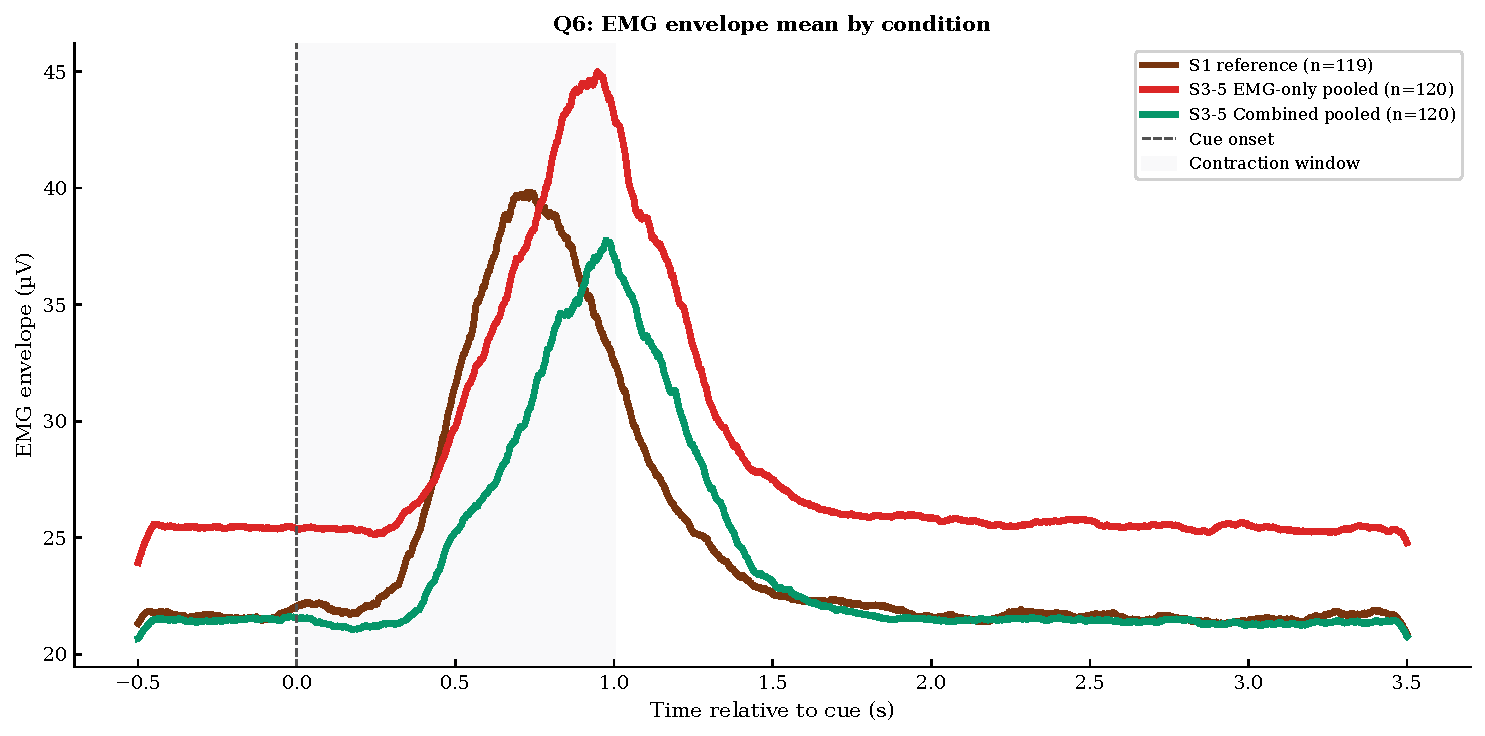
\includegraphics[width=\textwidth]{result_figures/q6_emg_means_by_condition.pdf}
  \caption{\gls{emg} envelope mean by condition: Session~1 reference ($n = \num{119}$), Sessions 3 to 5 EMG-only pooled ($n = \num{120}$), Sessions 3 to 5 Combined pooled ($n = \num{120}$). Dashed vertical line marks cue onset. Shaded region marks the \SI{1.0}{\second} contraction window.}
  \label{fig:q6-emg-means}
\end{figure}

The noise floor was $\num{21.70} \pm \num{0.99}$\,\si{\micro\volt} \gls{rms} for the Session~1 reference, $\num{25.49} \pm \num{13.76}$\,\si{\micro\volt} for the EMG-only block, and $\num{21.49} \pm \num{5.93}$\,\si{\micro\volt} for the Combined block. The EMG-only pooled mean was \SI{3.79}{\micro\volt} above the Session~1 reference. The Combined pooled mean was \SI{0.21}{\micro\volt} below the Session~1 reference. Contraction \gls{rms} was $\num{32.17} \pm \num{4.98}$\,\si{\micro\volt} for the Session~1 reference, $\num{33.88} \pm \num{13.11}$\,\si{\micro\volt} for the EMG-only block, and $\num{27.85} \pm \num{6.15}$\,\si{\micro\volt} for the Combined block. \gls{snr} was $\num{3.32} \pm \num{1.34}$\,\si{\decibel} for the Session~1 reference, $\num{3.04} \pm \num{1.83}$\,\si{\decibel} for the EMG-only block, and $\num{2.35} \pm \num{1.51}$\,\si{\decibel} for the Combined block. Per-session values are reported in Section~\ref{sec:results-q7}. Figure~\ref{fig:q6-emg-bars} shows the per-condition scalar metric bars.

\begin{figure}[!htbp]
  \centering
  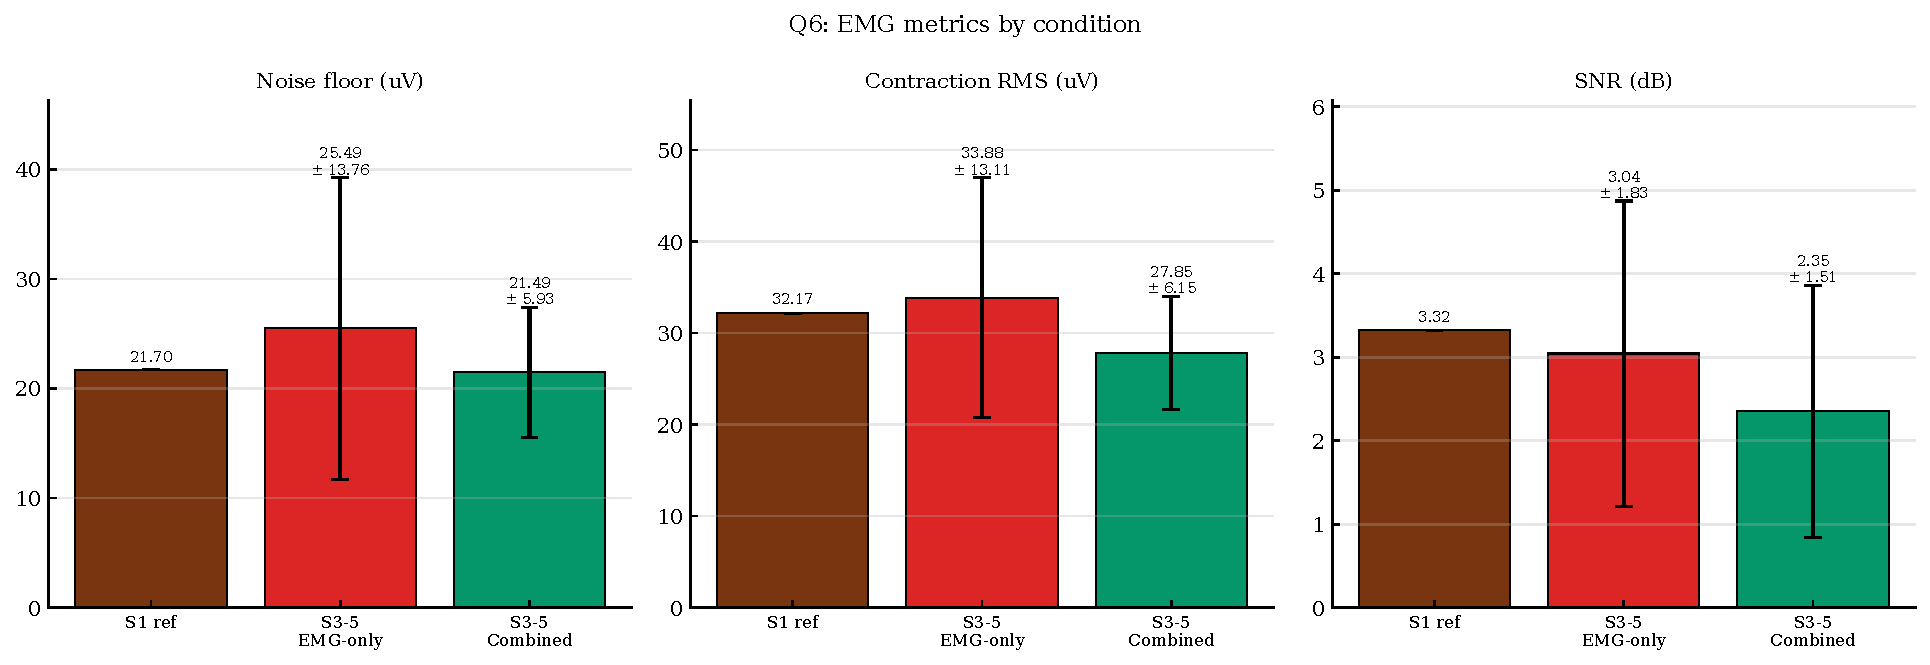
\includegraphics[width=\textwidth]{result_figures/q6_emg_metric_bars.pdf}
  \caption{\gls{emg} scalar metrics by condition: noise floor, contraction \gls{rms}, and \gls{snr}. Bars show the Session~1 reference value alongside the Sessions 3 to 5 EMG-only, and Combined block means. Pooled means span $n = \num{120}$ epochs per block, with $\pm 1$ SD error bars. The Session~1 reference is a single-session value ($n = \num{119}$). Per-epoch SDs are reported in Section~\ref{sec:results-q1}.}
  \label{fig:q6-emg-bars}
\end{figure}


Figure~\ref{fig:q6-emg-psd} shows the \gls{emg} \gls{psd} per condition. The Combined trace shows elevated chain-noise power below approximately \SI{1.5}{\hertz} relative to the EMG-only and S1 reference traces. The fraction of bins where chain-noise power exceeded the S1 reference level by more than \SI{3}{\decibel} was \SI{9.1}{\percent} for the Combined block and \SI{0.0}{\percent} for the EMG-only block. Table~\ref{tab:q6-emg-metrics} summarizes the per-condition metrics.

\begin{figure}[!htbp]
  \centering
  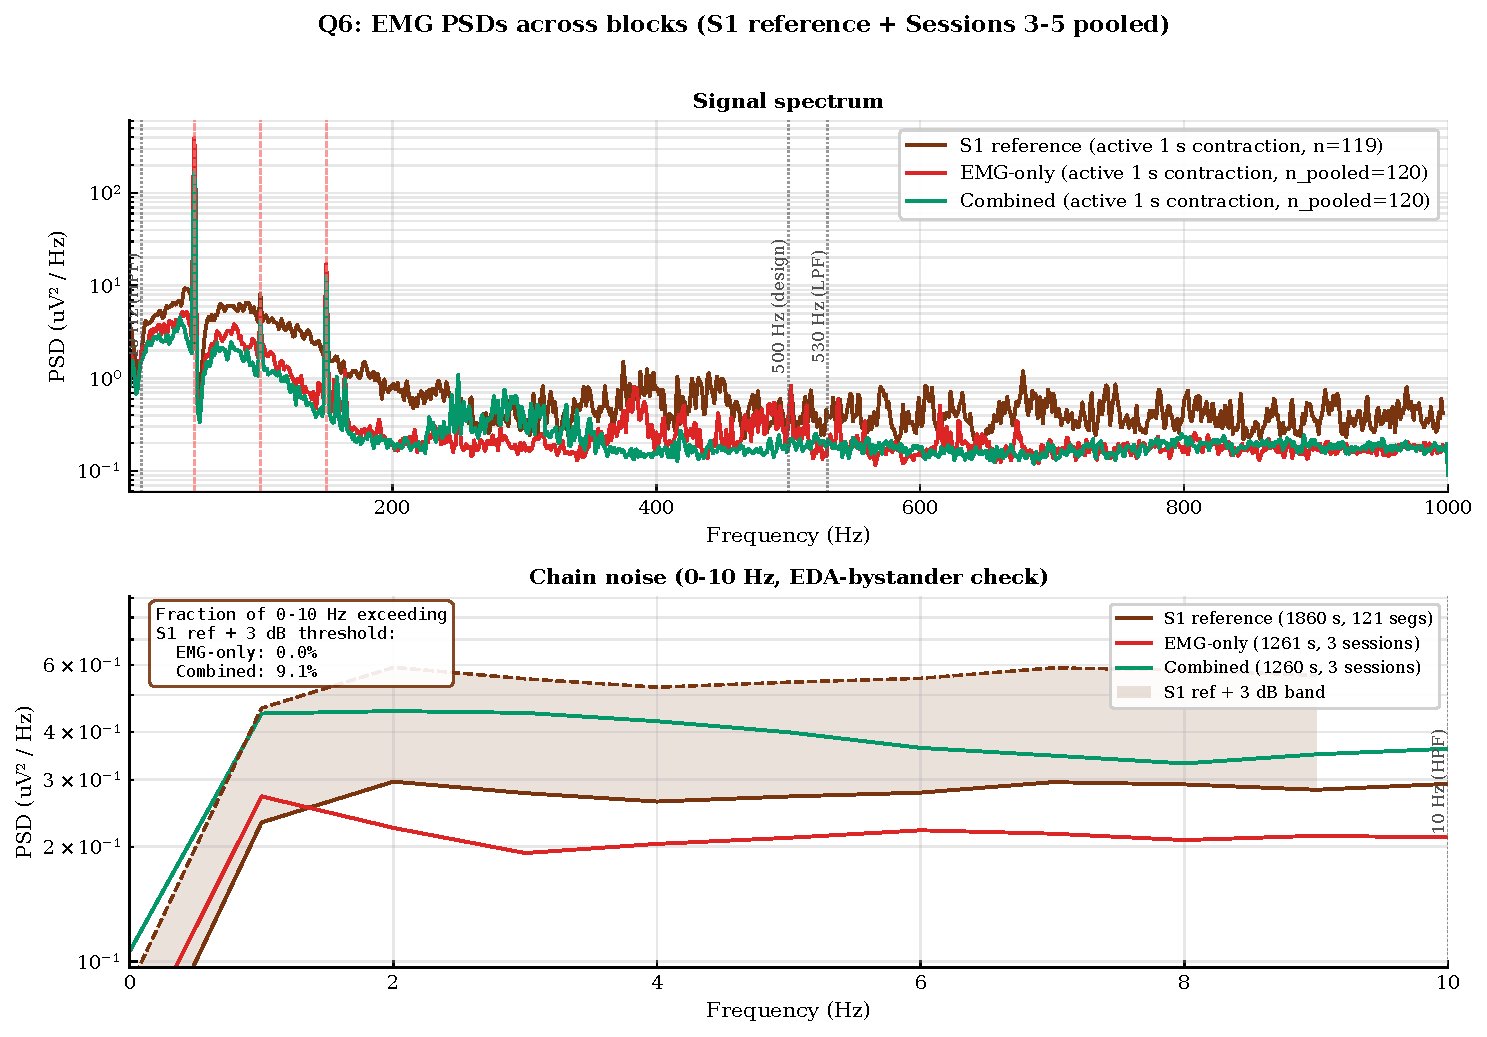
\includegraphics[width=\textwidth]{result_figures/q6_emg_psd.pdf}
  \caption{\gls{emg} \gls{psd} by condition: Session~1 reference, Sessions 3 to 5 EMG-only pooled, Sessions 3 to 5 Combined pooled. Top panel: signal spectrum from the active \SI{1}{\second} contraction window. Bottom panel: chain-noise spectrum from the cue-masked windows, restricted to the \SIrange{0}{10}{\hertz} band to highlight low-frequency \gls{eda} bystander effects. Vertical lines on the top panel mark the analog \gls{hpf} cutoff at \SI{10}{\hertz}, the design bandwidth at \SI{500}{\hertz}, and the analog \gls{lpf} cutoff at \SI{530}{\hertz}.}
  \label{fig:q6-emg-psd}
\end{figure}

\begin{table}[!htbp]
  \centering
  \caption{\gls{emg} per-condition metrics, Sessions 3 to 5 pooled with the Session~1 reference. Mean $\pm$ SD across epochs.}
  \label{tab:q6-emg-metrics}
  \begin{tabular}{l c c c l}
    \toprule
    \textbf{Metric} & \textbf{S1 ref} & \textbf{EMG-only} & \textbf{Combined} & \textbf{Unit} \\
    \midrule
    Noise floor & $\num{21.70} \pm \num{0.99}$ & $\num{25.49} \pm \num{13.76}$ & $\num{21.49} \pm \num{5.93}$ & \si{\micro\volt} \\
    Contraction \gls{rms} & $\num{32.17} \pm \num{4.98}$ & $\num{33.88} \pm \num{13.11}$ & $\num{27.85} \pm \num{6.15}$ & \si{\micro\volt} \\
    \gls{snr} & $\num{3.32} \pm \num{1.34}$ & $\num{3.04} \pm \num{1.83}$ & $\num{2.35} \pm \num{1.51}$ & \si{\decibel} \\
    \addlinespace
    Above-3 dB exceedance below \SIrange{0}{10}{\hertz}\textsuperscript{a} & -- & \SI{0.0}{\percent} & \SI{9.1}{\percent} & -- \\
    \bottomrule
  \end{tabular}
  
  \vspace{0.5em}
  \footnotesize
  \textsuperscript{a}Fraction of bins where chain-noise power exceeded the S1 reference level by more than \SI{3}{\decibel}. Computed per block.
\end{table}
 
 
% Framing claim (V2 locked): No time-locked EMG envelope deviation is
% observed at EDA cues in two of three sessions (S3 and S5). RMS pre and
% post matched 2-s windows are equivalent within all sessions. Session 4
% shows an apparent downward deviation at +5 s, but with elevated session-wide
% noise floor (~43 µV) consistent with the S4 anomaly reported in §4.3.1.
% Pooled across S3-5, the deviation amplitude is within the noise.
% Cross-references:
%   Methods metric definitions: \autoref{sec:methods-q6b}
%   S4 elevated noise floor context: \autoref{sec:results-q7}
%
% Discussion (DO NOT include here):
%   S4 deviation as session-level drift not cue-locked (Thread Q7.3): §5.5.
%   Coupling asymmetry (EMG→EDA real, EDA→EMG null) (Thread CrossQ.1): §5.1.
 
\FloatBarrier
 
\subsection{Q6b - EMG Response at EDA Cues}
\label{sec:results-q6b}

This section reports the cue-locked analysis of the \gls{emg} signal at \gls{eda} cues, addressing the inverse direction to the analysis in Section~\ref{sec:results-q5b}. Figure~\ref{fig:q6b-emg-by-session} shows the \gls{emg} envelope time-locked to \gls{eda} cues in the EDA-only block of Sessions 3 to 5, where no \gls{emg} stimulus was delivered. A downward deflection is visible in the Session~4 panel. The Session~3, Session~5, and pooled traces show no clear deflection. Deviation amplitude and deviation latency are defined in Section~\ref{sec:q6b_emg_at_eda_cues}. Positive amplitude indicates an upward rise of the envelope above baseline. The Q6b convention is the inverse of the Q5b convention. Pooled across the three sessions ($n = \num{30}$ epochs), the deviation amplitude was $-\num{2.99} \pm \num{7.12}$\,\si{\micro\volt} and the deviation latency was $\num{4.390} \pm \num{1.170}$\,\si{\second}. Pre-cue and post-cue \gls{rms} measured over matched 2-second windows were $\num{25.14} \pm \num{13.50}$\,\si{\micro\volt} and $\num{24.98} \pm \num{13.58}$\,\si{\micro\volt} respectively. The inter-cue interval was \SI{60}{\second} across all sessions.

\begin{figure}[!htbp]
  \centering
  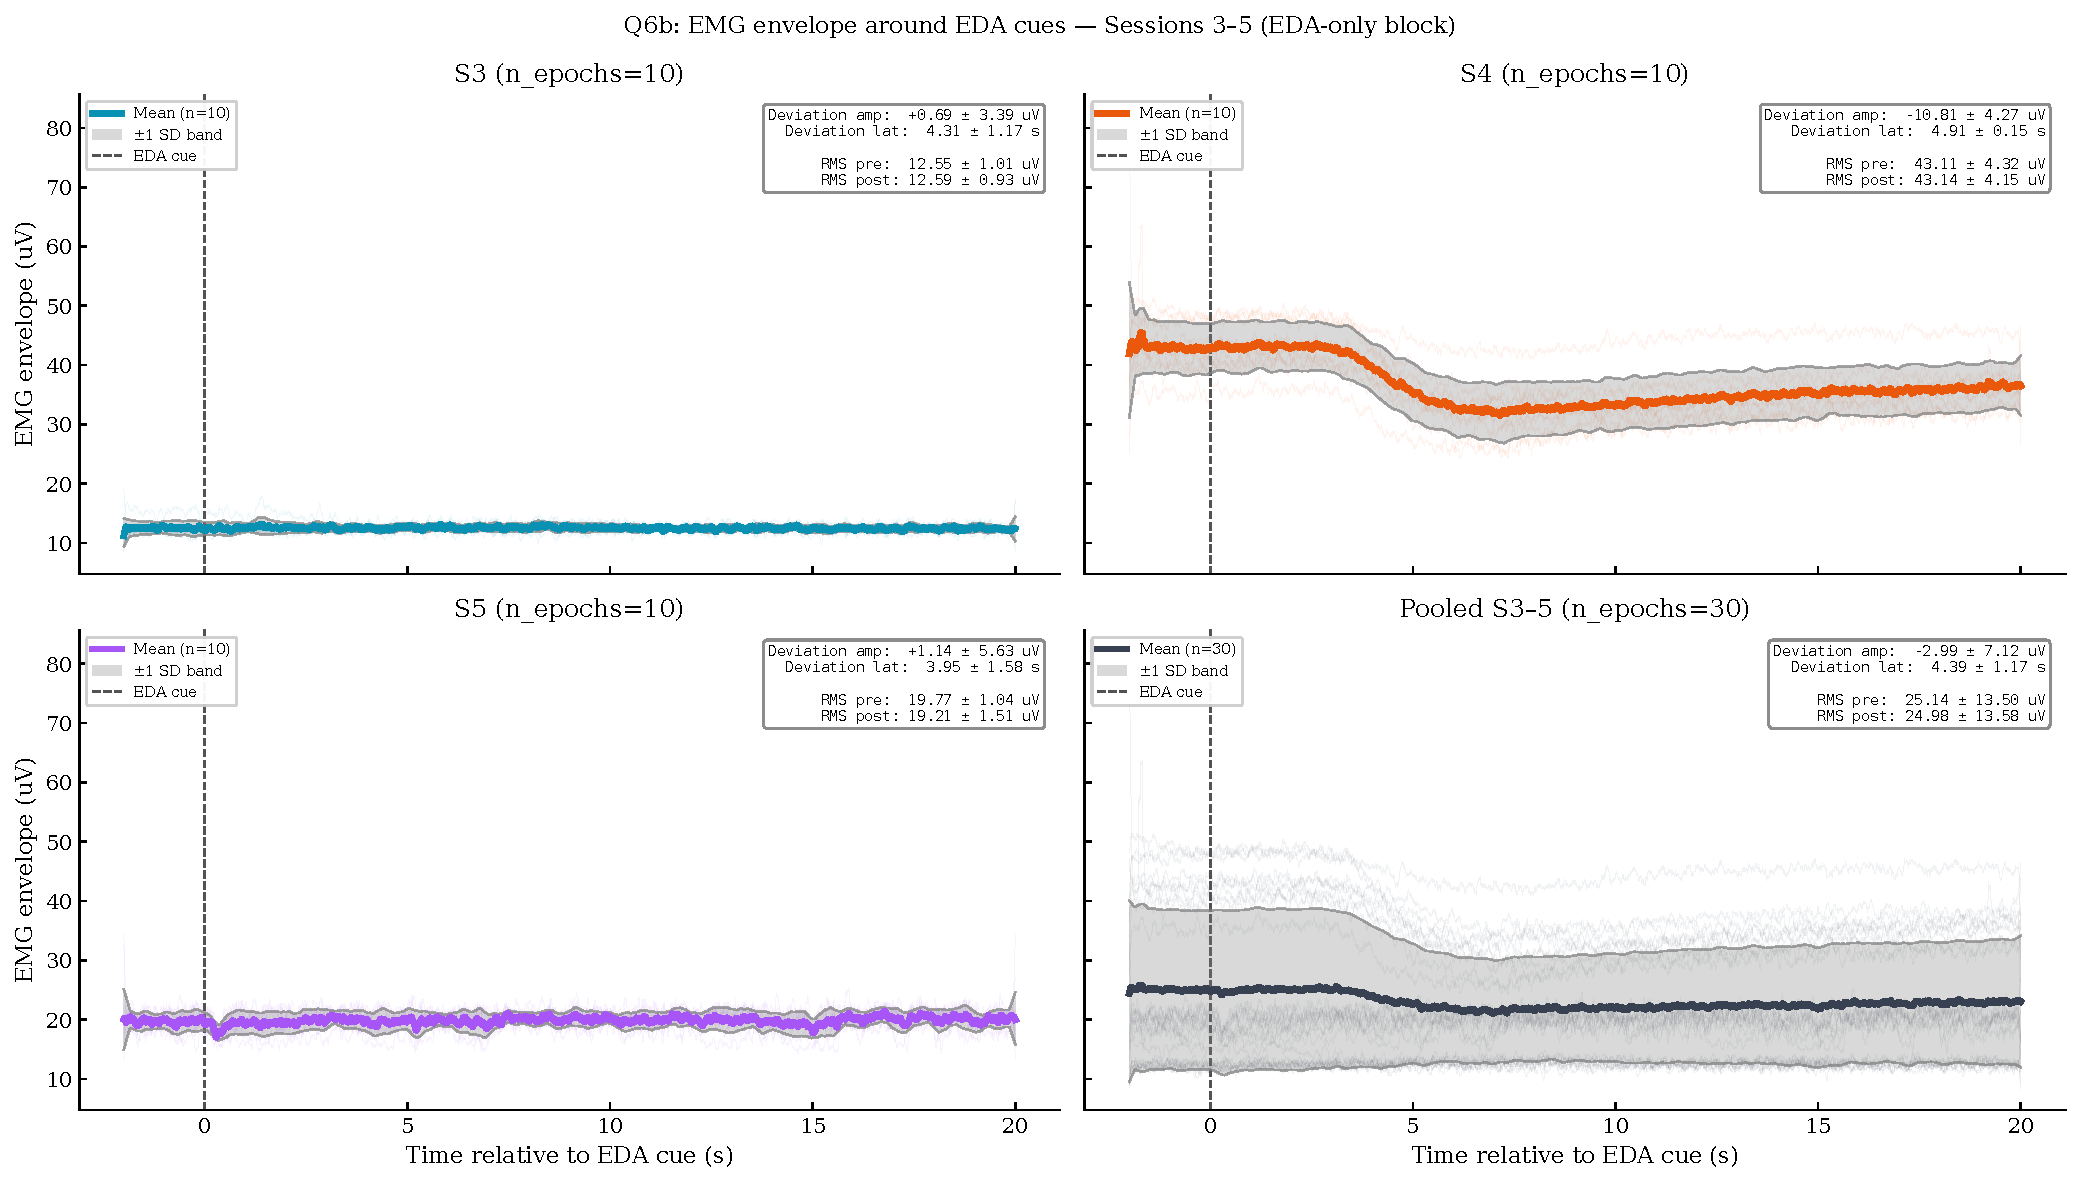
\includegraphics[width=\textwidth]{result_figures/q6b_emg_around_eda_cue_summary.pdf}
  \caption{\gls{emg} envelope around \gls{eda} cues in the EDA-only block of Sessions 3 to 5. Top row: Sessions~3 (left) and~4 (right). Bottom row: Session~5 (left) and pooled S3 to S5 (right). Each panel shows the mean signal (solid line) and individual epochs (light traces) with the grey band marking $\pm 1$ SD. The vertical line at $t = 0$ marks the \gls{eda} cue onset. Insets report deviation amplitude, deviation latency, and \gls{rms} before and after the cue.}
  \label{fig:q6b-emg-by-session}
\end{figure}

Per-session deviation amplitude was $+\num{0.69} \pm \num{3.39}$\,\si{\micro\volt} for S3, $-\num{10.81} \pm \num{4.27}$\,\si{\micro\volt} for S4, and $+\num{1.14} \pm \num{5.63}$\,\si{\micro\volt} for S5 ($n = \num{10}$ epochs each). Per-session deviation latency was $\num{4.309} \pm \num{1.169}$\,\si{\second} for S3, $\num{4.912} \pm \num{0.147}$\,\si{\second} for S4, and $\num{3.948} \pm \num{1.579}$\,\si{\second} for S5. Per-session pre-cue and post-cue \gls{rms} were $\num{12.55} \pm \num{1.01}$ and $\num{12.59} \pm \num{0.93}$\,\si{\micro\volt} for S3, $\num{43.11} \pm \num{4.32}$ and $\num{43.14} \pm \num{4.15}$\,\si{\micro\volt} for S4, and $\num{19.77} \pm \num{1.04}$ and $\num{19.21} \pm \num{1.51}$\,\si{\micro\volt} for S5. Per-session noise floor context is reported in Section~\ref{sec:results-q7}. Table~\ref{tab:q6b-metrics} summarizes the per-session and pooled metrics.

\begin{table}[!htbp]
  \centering
  \caption{Per-session and pooled \gls{emg} metrics around \gls{eda} cues, Sessions 3 to 5 (EDA-only block). Deviation amplitude is signed. Positive values indicate an upward rise above baseline.}
  \label{tab:q6b-metrics}
  \begin{tabular}{l c c c c l}
    \toprule
    \textbf{Metric} & \textbf{S3} & \textbf{S4} & \textbf{S5} & \textbf{Pooled S3-5} & \textbf{Unit} \\
    \midrule
    $n$                  & \num{10} & \num{10} & \num{10} & \num{30} & --- \\
    Deviation amplitude  & $+\num{0.69}  \pm \num{3.39}$ & $-\num{10.81} \pm \num{4.27}$ & $+\num{1.14}  \pm \num{5.63}$ & $-\num{2.99} \pm \num{7.12}$ & \si{\micro\volt} \\
    Deviation latency    & $\num{4.309} \pm \num{1.169}$  & $\num{4.912} \pm \num{0.147}$  & $\num{3.948} \pm \num{1.579}$  & $\num{4.390} \pm \num{1.170}$  & \si{\second} \\
    \addlinespace
    \gls{rms} pre-cue    & $\num{12.55} \pm \num{1.01}$ & $\num{43.11} \pm \num{4.32}$ & $\num{19.77} \pm \num{1.04}$ & $\num{25.14} \pm \num{13.50}$ & \si{\micro\volt} \\
    \gls{rms} post-cue   & $\num{12.59} \pm \num{0.93}$ & $\num{43.14} \pm \num{4.15}$ & $\num{19.21} \pm \num{1.51}$ & $\num{24.98} \pm \num{13.58}$ & \si{\micro\volt} \\
    \bottomrule
  \end{tabular}
\end{table}


\FloatBarrier

% =============================================================================
% 4.3 Reproducibility and Quality Control (Q7 + folded QC opener)
%
% Single subsection covering per-session reproducibility across S3-5. The
% epoch-level contamination filter exclusion report is folded into §4.3.1's
% opener as a methodological prelude before the per-session metrics.
% =============================================================================

\section{Reproducibility and Quality Control}
\label{sec:results-reproducibility}

This section reports the per-session reproducibility of \gls{emg} and \gls{eda} scalar metrics across the simultaneous-acquisition sessions. Between-session variability is reported for both modalities alongside the contamination filter exclusion summary. The data are drawn from Sessions~3 to~5.
 
% Framing claim (V2 locked): Both EMG and EDA metrics show between-session
% variability across Sessions 3-5. Session 4 is an outlier in both modalities
% in opposite directions: elevated EMG noise floor and contraction RMS,
% reduced EDA baseline conductance (SCL), but cleanest EDA SNR_circuit.
% Per-session signal traces show the S4 EMG-only block sits at substantially
% higher amplitude than its Combined block.
% Cross-references:
%   Methods Q7 description: \autoref{sec:methods-q7}
%   Methods contamination filter: \autoref{sec:methods-contamination-filter}
%   Pooled S3-5 EMG metrics: \autoref{sec:results-q6}
%   Pooled S3-5 EDA metrics: \autoref{sec:results-q5}
%
% Discussion (DO NOT include here):
%   S4 cross-modality asymmetry interpretation (Thread Q7.3): §5.5.
%   SCR amplitude reproducibility, S4 reverses (Thread Q5.1): §5.5.
%   SNR_circuit cross-session variability (Thread Q7.2): §5.5.

\subsection{Q7 - Per-Session Reproducibility}
\label{sec:results-q7}

Figure~\ref{fig:q7-per-session-traces} shows the per-session signal traces across blocks for both modalities.

\begin{figure}[!htbp]
  \centering
  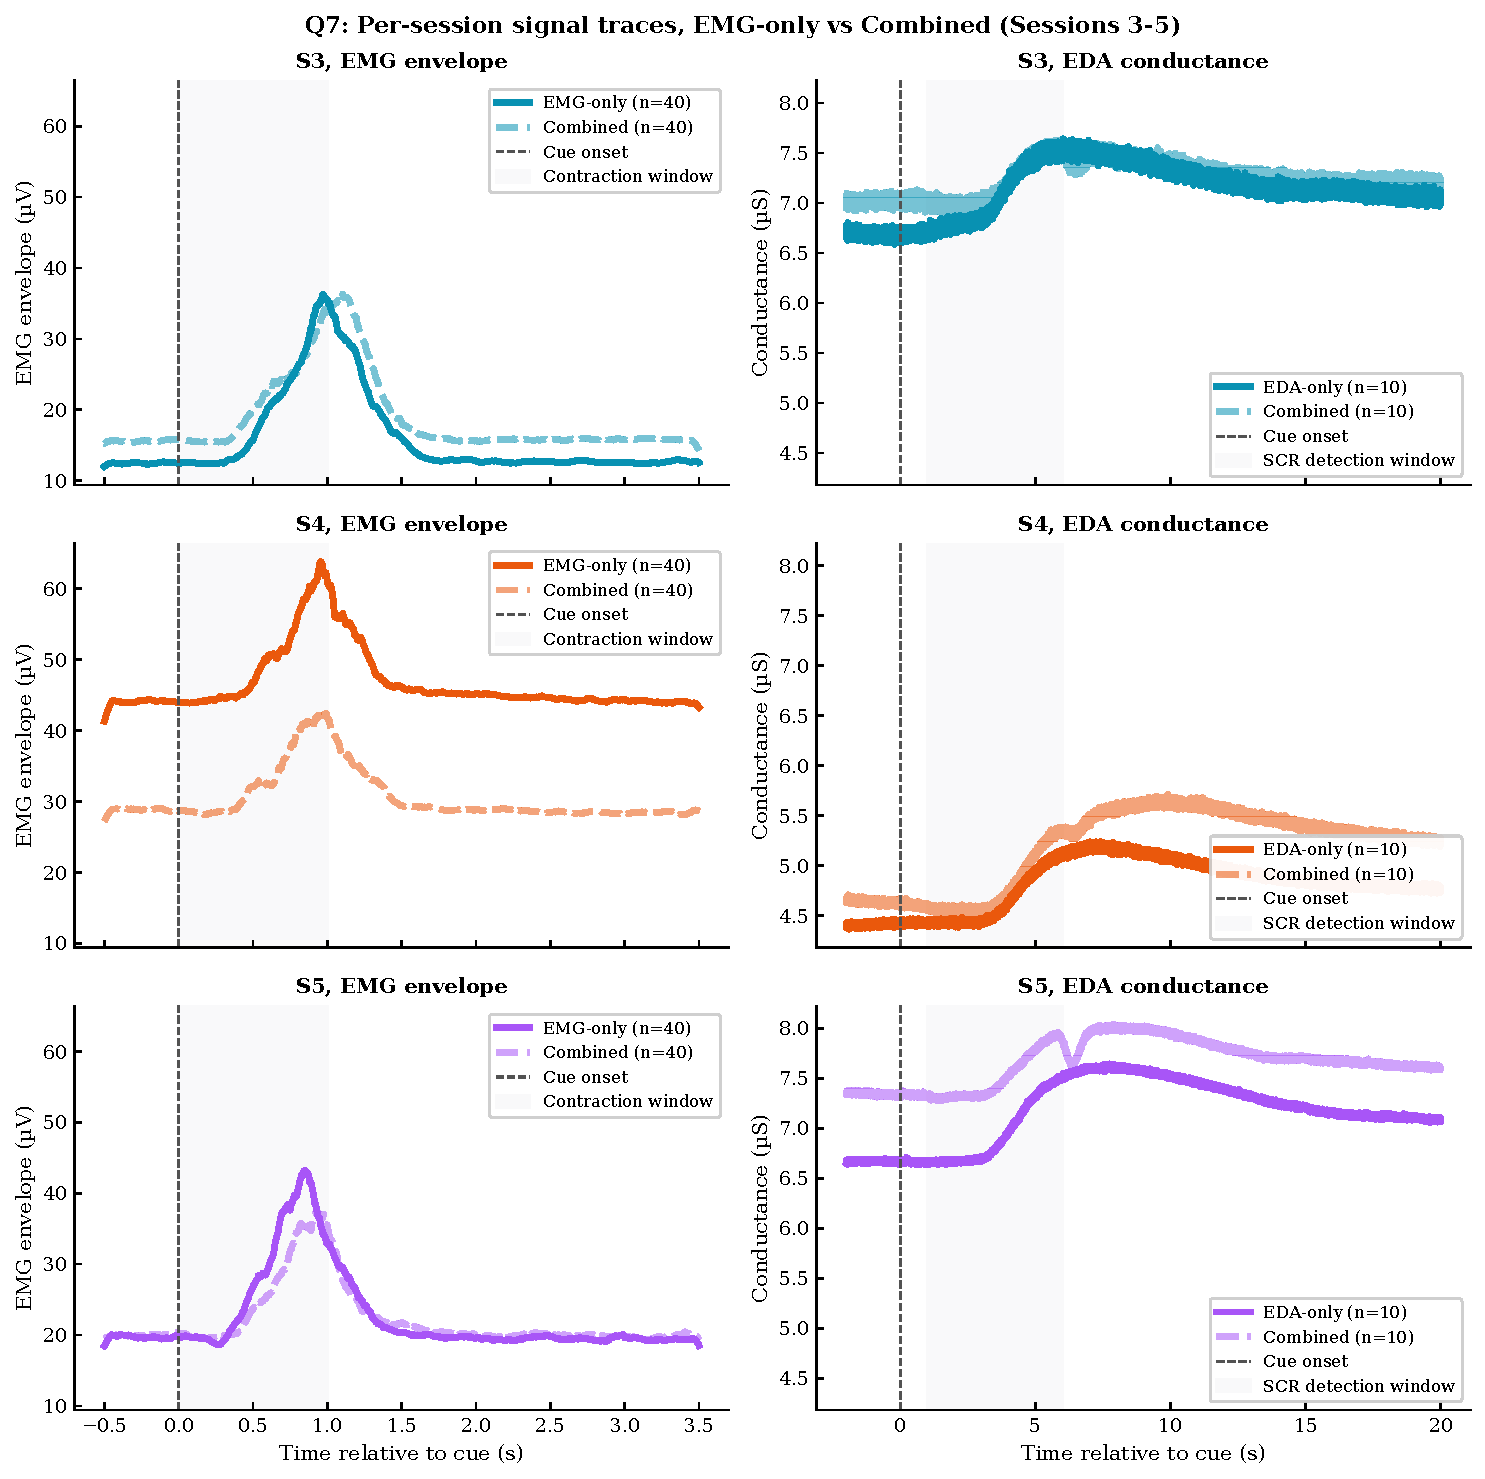
\includegraphics[width=\textwidth]{result_figures/q7_per_session_traces.pdf}
  \caption{Per-session signal traces across blocks. Rows: Sessions 3, 4, and 5. Columns: \gls{emg} envelope (left) and \gls{eda} conductance (right). Each panel overlays two signal means: solid for the single-modality block and dashed for the Combined block. Line color encodes the session. The y-axis is shared per column. Dashed vertical line at $t = 0$ marks the cue onset. Shaded region in the \gls{emg} column marks the \SI{1.0}{\second} contraction window. Shaded region in the \gls{eda} column marks the \SIrange{1}{6}{\second} \gls{scr} detection window.}
  \label{fig:q7-per-session-traces}
\end{figure}

\FloatBarrier

\subsubsection{EMG}
\label{sec:results-q7-emg}

The contamination filter (Section~\ref{sec:emg_processing}) rejected \num{1} of \num{360} \gls{emg} epochs across all session-blocks (\num{0.28}\,\%). Per-block thresholds, computed as twice the median pre-cue \gls{rms} per session-block, ranged from \SI{24.88}{\micro\volt} (S3 EMG-only) to \SI{87.73}{\micro\volt} (S4 EMG-only). Table~\ref{tab:q7-qc-filter} reports the per-session-block exclusion counts and thresholds. 

\begin{table}[!htbp]
  \centering
  \caption{Contamination filter exclusion summary across all \gls{emg} session-blocks. Threshold computed as $2 \times \operatorname{median}(\text{pre-cue \gls{rms}})$ per session-block.}
  \label{tab:q7-qc-filter}
  \begin{tabular}{l c c}
    \toprule
    \textbf{Session-block} & \textbf{Excluded / Total} & \textbf{Threshold (\si{\micro\volt})} \\
    \midrule
    S1            & \num{1}/\num{120} & \num{43.22} \\
    \addlinespace
    S3 EMG-only   & \num{0}/\num{40}  & \num{24.88} \\
    S3 Combined   & \num{0}/\num{40}  & \num{31.65} \\
    S4 EMG-only   & \num{0}/\num{40}  & \num{87.73} \\
    S4 Combined   & \num{0}/\num{40}  & \num{57.48} \\
    S5 EMG-only   & \num{0}/\num{40}  & \num{40.64} \\
    S5 Combined   & \num{0}/\num{40}  & \num{40.10} \\
    \midrule
    \textbf{Total} & \textbf{\num{1}/\num{360}} (\num{0.28}\,\%) & --- \\
    \bottomrule
  \end{tabular}
\end{table}

Figure~\ref{fig:q7-emg-bars} shows the per-session \gls{emg} scalar metrics across both blocks, and Figure~\ref{fig:q7-emg-by-block} shows the same metrics as block trajectories from EMG-only to Combined. The noise floor was \SI{12.50}{\micro\volt} for S3 EMG-only and \SI{15.63}{\micro\volt} for S3 Combined, \SI{44.14}{\micro\volt} for S4 EMG-only and \SI{28.86}{\micro\volt} for S4 Combined, and \SI{19.81}{\micro\volt} for S5 EMG-only and \SI{19.97}{\micro\volt} for S5 Combined. Contraction \gls{rms} was \SI{21.10}{\micro\volt} and \SI{22.39}{\micro\volt} for S3 across the two blocks, \SI{50.46}{\micro\volt} and \SI{33.88}{\micro\volt} for S4, and \SI{30.07}{\micro\volt} and \SI{27.28}{\micro\volt} for S5. \gls{snr} was \SI{4.44}{\decibel} and \SI{3.06}{\decibel} for S3, \SI{1.15}{\decibel} and \SI{1.39}{\decibel} for S4, and \SI{3.55}{\decibel} and \SI{2.61}{\decibel} for S5. Table~\ref{tab:q7-emg-metrics} summarizes the per-session per-block \gls{emg} metrics. Pooled values across Sessions 3 to 5 are reported in Section~\ref{sec:results-q6}.

\begin{figure}[!htbp]
  \centering
  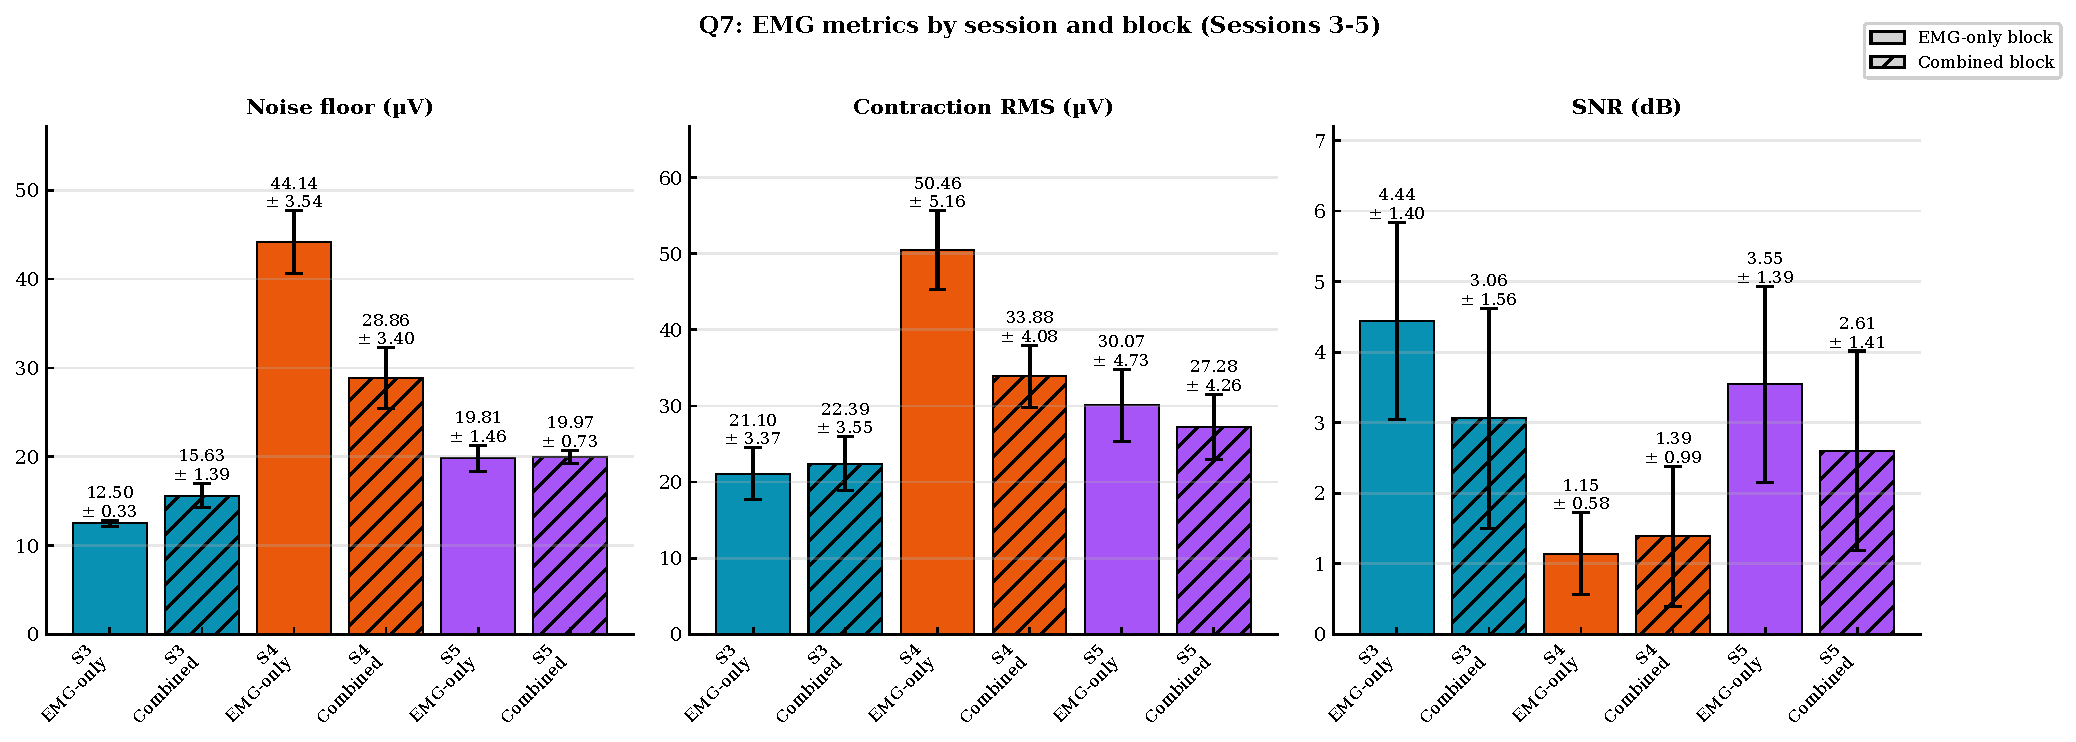
\includegraphics[width=\textwidth]{result_figures/q7_emg_metric_bars.pdf}
  \caption{Per-session \gls{emg} metrics across Sessions 3 to 5 EMG-only and Combined blocks. Three panels: noise floor, contraction \gls{rms}, and \gls{snr}. Bar color encodes session (S3, S4, S5). Hatch encodes block (solid for single-modality, hatched for Combined). Error bars show $\pm 1$ SD across each session-block's clean epochs.}
  \label{fig:q7-emg-bars}
\end{figure}

\begin{figure}[!htbp]
  \centering
  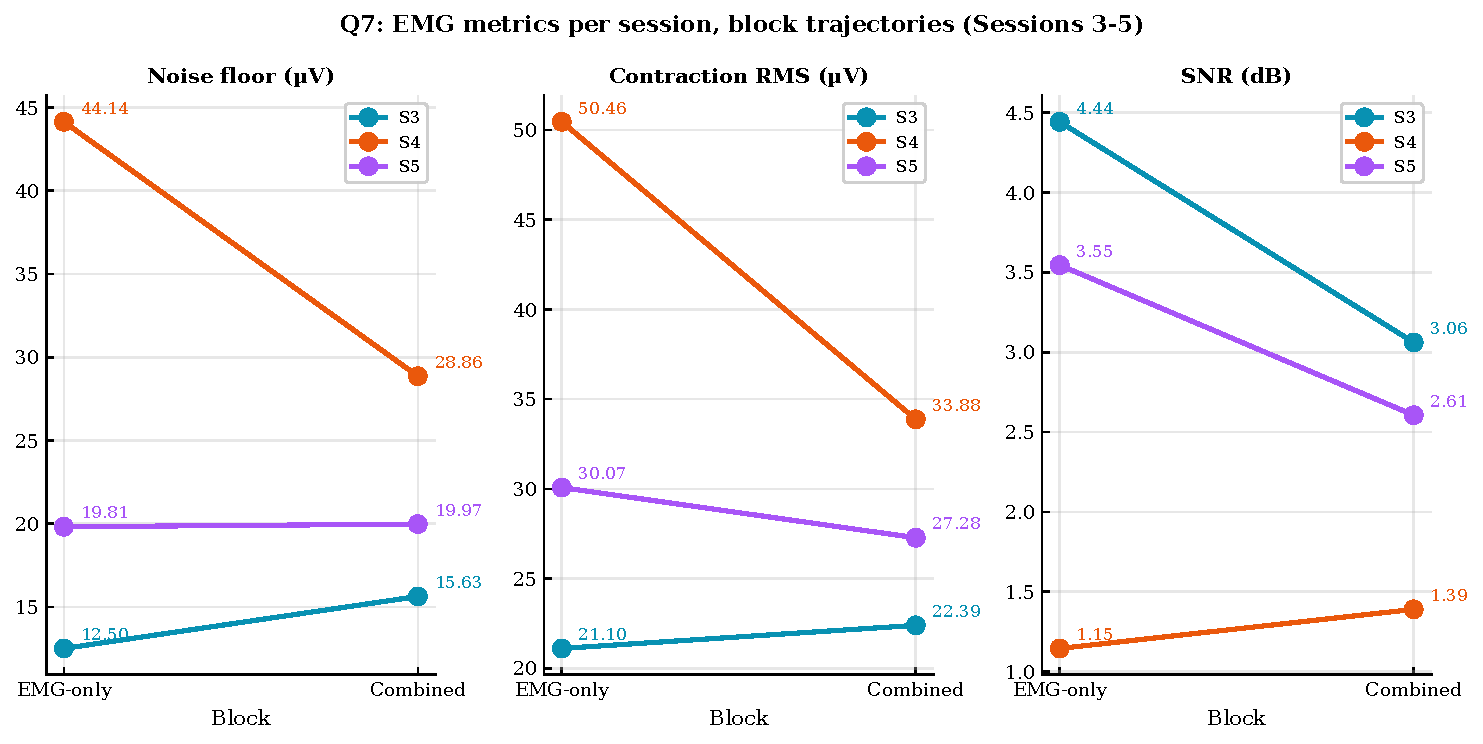
\includegraphics[width=\textwidth]{result_figures/q7_emg_by_block.pdf}
  \caption{\gls{emg} metrics per session as block trajectories from EMG-only to Combined. Three panels: noise floor, contraction \gls{rms}, and \gls{snr}. Each line connects the two block measurements for the same session. Line color encodes the session.}
  \label{fig:q7-emg-by-block}
\end{figure}

\begin{table}[!htbp]
  \centering
  \caption{Per-session per-block \gls{emg} metrics, Sessions 3 to 5. Mean $\pm$ SD across each session-block's clean epochs ($n = \num{40}$ per block).}
  \label{tab:q7-emg-metrics}
  \begin{tabular}{l l c c c}
    \toprule
    \textbf{Session} & \textbf{Block} & \textbf{NF (\si{\micro\volt})} & \textbf{Contr \gls{rms} (\si{\micro\volt})} & \textbf{\gls{snr} (\si{\decibel})} \\
    \midrule
    S3 & EMG-only & $\num{12.50} \pm \num{0.33}$ & $\num{21.10} \pm \num{3.37}$ & $\num{4.44} \pm \num{1.40}$ \\
    S3 & Combined & $\num{15.63} \pm \num{1.39}$ & $\num{22.39} \pm \num{3.55}$ & $\num{3.06} \pm \num{1.56}$ \\
    \addlinespace
    S4 & EMG-only & $\num{44.14} \pm \num{3.54}$ & $\num{50.46} \pm \num{5.16}$ & $\num{1.15} \pm \num{0.58}$ \\
    S4 & Combined & $\num{28.86} \pm \num{3.40}$ & $\num{33.88} \pm \num{4.08}$ & $\num{1.39} \pm \num{0.99}$ \\
    \addlinespace
    S5 & EMG-only & $\num{19.81} \pm \num{1.46}$ & $\num{30.07} \pm \num{4.73}$ & $\num{3.55} \pm \num{1.39}$ \\
    S5 & Combined & $\num{19.97} \pm \num{0.73}$ & $\num{27.28} \pm \num{4.26}$ & $\num{2.61} \pm \num{1.41}$ \\
    \bottomrule
  \end{tabular}
\end{table}

\FloatBarrier

\subsubsection{EDA}
\label{sec:results-q7-eda}

Figure~\ref{fig:q7-eda-bars} shows the per-session \gls{eda} scalar metrics across both blocks: \gls{scl}, \gls{scr} amplitude, \gls{snr}$_{\text{circuit}}$, and \gls{snr}$_{\text{local}}$. Figure~\ref{fig:q7-eda-by-block} shows the same metrics as block trajectories from EDA-only to Combined. \gls{scl} was \SI{6.689}{\micro\siemens} and \SI{7.020}{\micro\siemens} for S3 across the two blocks, \SI{4.412}{\micro\siemens} and \SI{4.640}{\micro\siemens} for S4, and \SI{6.667}{\micro\siemens} and \SI{7.343}{\micro\siemens} for S5. \gls{scr} amplitude was \SI{0.830}{\micro\siemens} and \SI{0.589}{\micro\siemens} for S3, \SI{0.701}{\micro\siemens} and \SI{0.802}{\micro\siemens} for S4, and \SI{0.870}{\micro\siemens} and \SI{0.674}{\micro\siemens} for S5. \gls{snr}$_{\text{circuit}}$ was \SI{7.33}{\decibel} and \SI{4.35}{\decibel} for S3, \SI{12.01}{\decibel} and \SI{13.18}{\decibel} for S4, and \SI{3.24}{\decibel} and \SI{1.03}{\decibel} for S5. \gls{snr}$_{\text{local}}$ was \SI{19.57}{\decibel} and \SI{15.83}{\decibel} for S3, \SI{25.26}{\decibel} and \SI{25.49}{\decibel} for S4, and \SI{30.46}{\decibel} and \SI{27.37}{\decibel} for S5. Pooled values across Sessions 3 to 5 are reported in Section~\ref{sec:results-q5}.


\begin{figure}[!htbp]
  \centering
  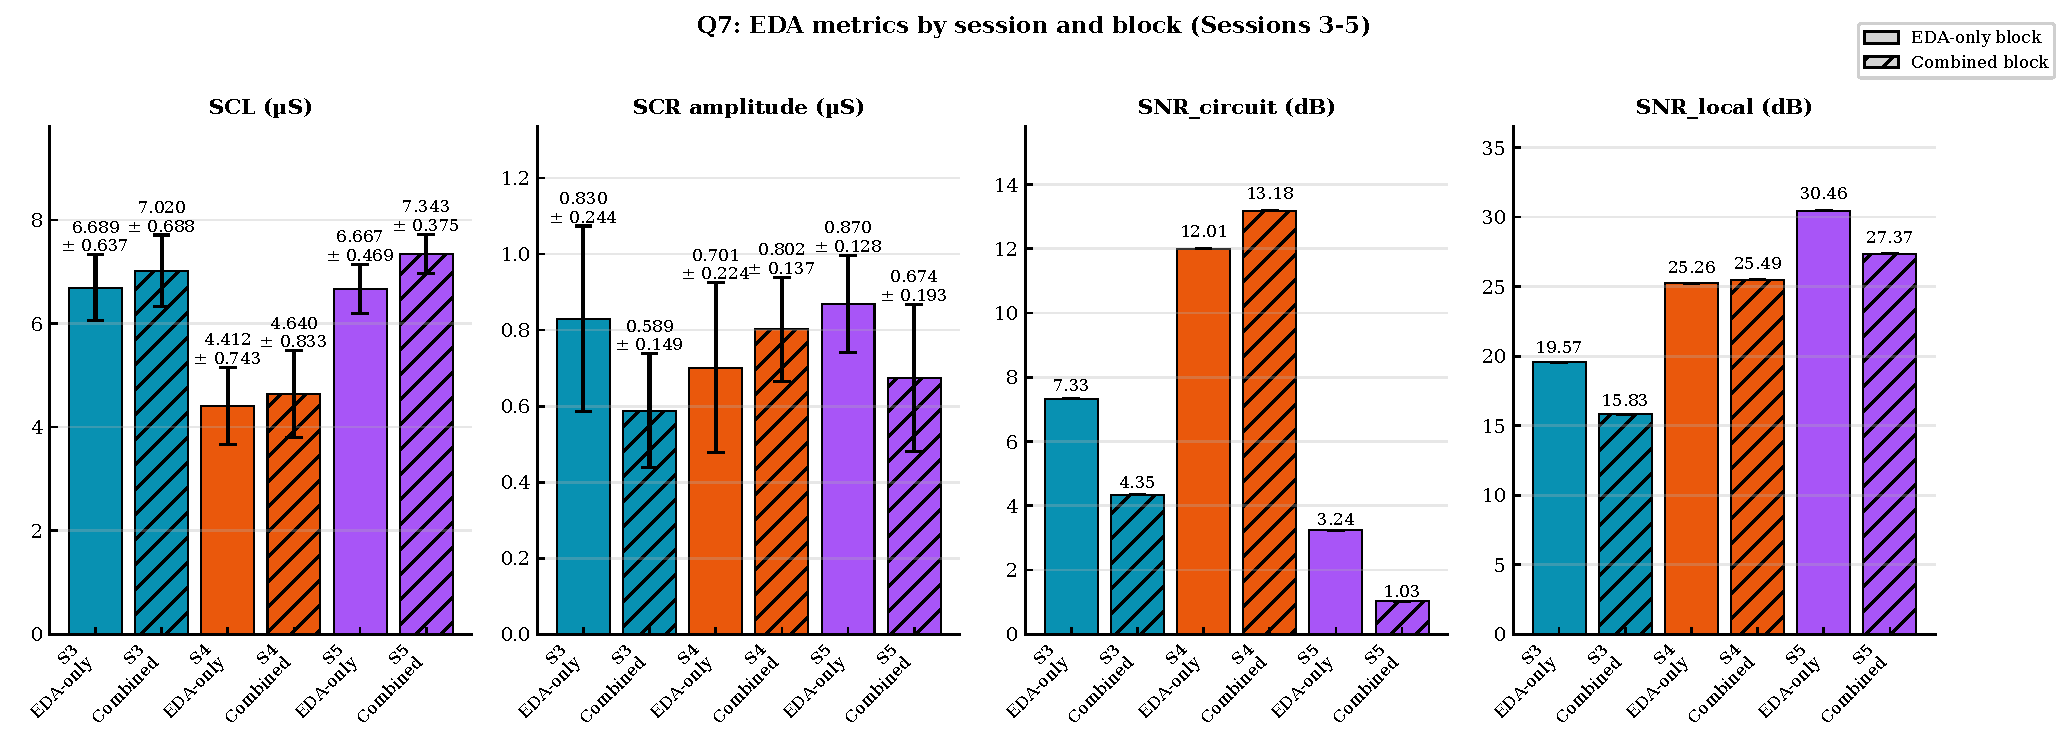
\includegraphics[width=\textwidth]{result_figures/q7_eda_metric_bars.pdf}
  \caption{Per-session \gls{eda} metrics across Sessions 3 to 5 EDA-only and Combined blocks. Four panels: \gls{scl}, \gls{scr} amplitude, \gls{snr}$_{\text{circuit}}$, and \gls{snr}$_{\text{local}}$. Bar color encodes the session. Hatch encodes block. Error bars on \gls{scl} and \gls{scr} amplitude show $\pm 1$ SD across each session-block's epochs. \gls{snr} bars are session-level scalars without per-epoch SD.}
  \label{fig:q7-eda-bars}
\end{figure}

\begin{figure}[!htbp]
  \centering
  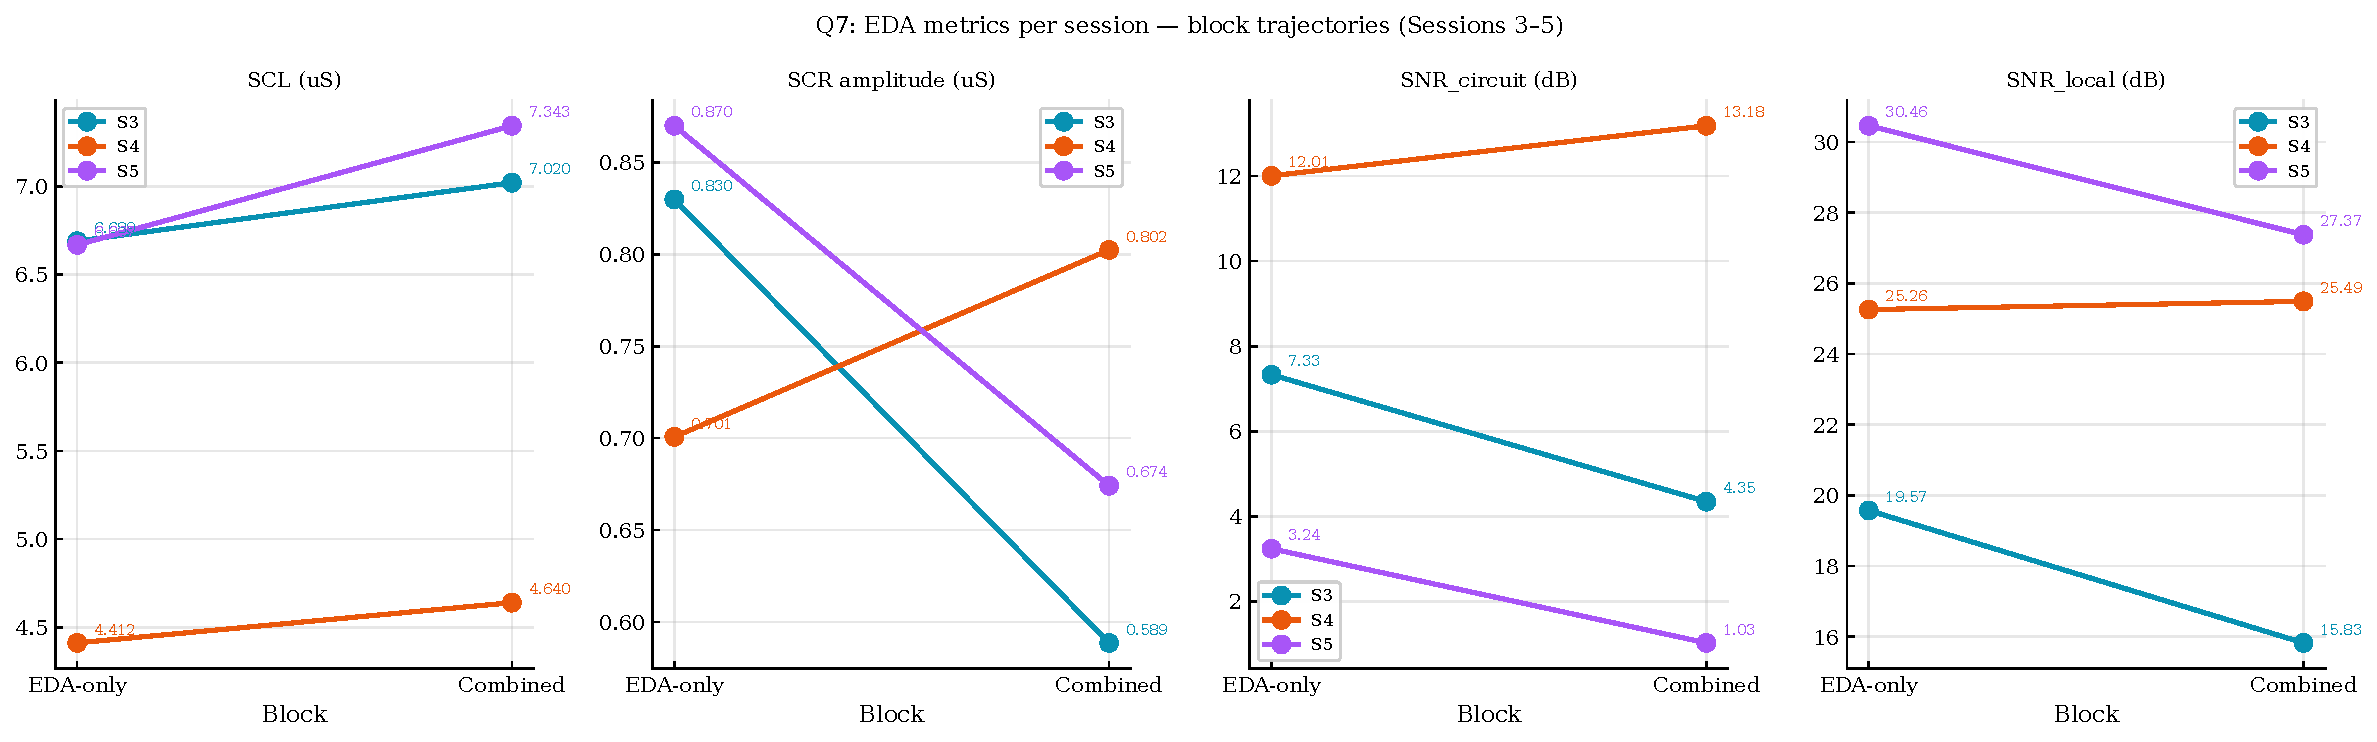
\includegraphics[width=\textwidth]{result_figures/q7_eda_by_block.pdf}
  \caption{\gls{eda} metrics per session as block trajectories from EDA-only to Combined. Four panels: \gls{scl}, \gls{scr} amplitude, \gls{snr}$_{\text{circuit}}$, and \gls{snr}$_{\text{local}}$. Each line connects the two block measurements for the same session. Line color encodes the session.}
  \label{fig:q7-eda-by-block}
\end{figure}

Tables~\ref{tab:q7-eda-signal} and~\ref{tab:q7-eda-noise-snr} report the per-session per-block \gls{eda} measurements for Sessions 3 to 5. Table~\ref{tab:q7-eda-signal} groups the signal quantities, \gls{scl} and \gls{scr} amplitude. Table~\ref{tab:q7-eda-noise-snr} groups the noise floor and \gls{snr} metrics. The noise floor is reported under two conventions. $\sigma_{\text{local}}$ is computed from the \SI{2}{\second} pre-cue window per epoch and resolves block-level variation.$\sigma_{\text{session}}$ is computed from the 10-minute post-isolation stabilization recording captured before the test run and is therefore session-level rather than block-level.
\begin{table}[!htbp]
  \centering
  \caption{Per-session per-block \gls{eda} signal quantities, Sessions 3 to 5. Mean $\pm$ SD across each session-block's epochs ($n = \num{10}$ per block) for \gls{scl} and \gls{scr} amplitude.}
  \label{tab:q7-eda-signal}
  \begin{tabular}{l l c c}
    \toprule
    \textbf{Session} & \textbf{Block} & \textbf{\gls{scl} (\si{\micro\siemens})} & \textbf{\gls{scr} amp (\si{\micro\siemens})} \\
    \midrule
    S3 & EDA-only & $\num{6.689} \pm \num{0.637}$ & $\num{0.830} \pm \num{0.244}$ \\
    S3 & Combined & $\num{7.020} \pm \num{0.688}$ & $\num{0.589} \pm \num{0.149}$ \\
    \addlinespace
    S4 & EDA-only & $\num{4.412} \pm \num{0.743}$ & $\num{0.701} \pm \num{0.224}$ \\
    S4 & Combined & $\num{4.640} \pm \num{0.833}$ & $\num{0.802} \pm \num{0.137}$ \\
    \addlinespace
    S5 & EDA-only & $\num{6.667} \pm \num{0.469}$ & $\num{0.870} \pm \num{0.128}$ \\
    S5 & Combined & $\num{7.343} \pm \num{0.375}$ & $\num{0.674} \pm \num{0.193}$ \\
    \bottomrule
  \end{tabular}
\end{table}

\begin{table}[!htbp]
  \centering
  \caption{Per-session per-block \gls{eda} noise floor and \gls{snr} metrics, Sessions 3 to 5. $\sigma_{\text{local}}$ is the mean per-epoch detrended SD over the \SI{2}{\second} pre-cue window, per block. $\sigma_{\text{session}}$ is the SD of the linearly detrended 10-minute post-isolation stabilization recording, per session, and therefore takes one value per session. \gls{snr} values are session-block scalars without per-epoch SD.}
  \label{tab:q7-eda-noise-snr}
  \begin{tabular}{l l c c c c}
    \toprule
    \textbf{Session} & \textbf{Block} & \boldmath$\sigma_{\text{local}}$ \textbf{(\si{\micro\siemens})} & \boldmath$\sigma_{\text{session}}$ \textbf{(\si{\micro\siemens})} & \textbf{\gls{snr}$_{\text{local}}$ (\si{\decibel})} & \textbf{\gls{snr}$_{\text{circuit}}$ (\si{\decibel})} \\
    \midrule
    S3 & EDA-only & \num{0.087} & \multirow{2}{*}{\num{0.357}} & \num{19.57} & \num{7.33}  \\
    S3 & Combined & \num{0.095} &                                & \num{15.83} & \num{4.35}  \\
    \addlinespace
    S4 & EDA-only & \num{0.038} & \multirow{2}{*}{\num{0.176}} & \num{25.26} & \num{12.01} \\
    S4 & Combined & \num{0.043} &                                & \num{25.49} & \num{13.18} \\
    \addlinespace
    S5 & EDA-only & \num{0.026} & \multirow{2}{*}{\num{0.599}} & \num{30.46} & \num{3.24}  \\
    S5 & Combined & \num{0.029} &                                & \num{27.37} & \num{1.03}  \\
    \bottomrule
  \end{tabular}
\end{table}

\FloatBarrier

\begin{comment}    
\begin{itemize}
    \item Build your result
    \item What's new?
    \item The result itself
\end{itemize}
\end{comment}